%\documentclass[uplatex,dvipdfmx]{jsarticle}
 
%\usepackage[dvipdfmx]{graphicx}
%\usepackage{graphicx}
%\usepackage{mathtools}
%\usepackage{cancel}
%\usepackage{amsmath,amssymb}
%\usepackage{cases}
%\usepackage{bm}

%\usepackage{here}
%\usepackage{colortbl}
%\usepackage{feynmf}

%\newcommand{\Slash}[1]{{\ooalign{\hfil/\hfil\crcr\(#1\)}}}

%\begin{document}

\newpage
%\section{実験}

\subsection{寿命測定のための銅板標的}

寿命測定に用いた銅板標的を図~\ref{tar_cu} に示す.
これは厚さ$0.6~\mathrm{mm} \times$ 横$280~\mathrm{mm} \times$ 縦$120~\mathrm{mm}$ の銅板を木枠に固定したものである.銅板の縦横の長さはビームプロファイルから計算されるビームの広がりに対して約$3\sigma$ になるように決めた.また厚さは$4~\mathrm{MeV}$ ミューオンが銅板厚み方向の中心付近で止まるようなものを選んだ.

\subsection{$g$ 因子測定のための磁場装置}

$g$ 因子測定に用いた磁場印加標的を図~\ref{tar_mag} に示す.
厚さ$0.6~\mathrm{mm} \times$ 横$80~\mathrm{mm} \times$ 縦$60~\mathrm{mm}$ の銅板を,呼び径$200~\mathrm{mm}$ の塩化ビニルパイプの中心にくるように紐で吊るした.銅板の縦横の大きさはミューオンビームの広がりに対して約$1\sigma$ の大きさになるように決めた.パイプ内側に計36 個の永久磁石を接着剤で貼り付け,テープで補強した(磁石の配置については後述).永久磁石にはセラミック磁石 (Y25) を用いており,磁石一個あたりの大きさは厚さ$9~\mathrm{mm} \times$ 横幅$10~\mathrm{mm} \times$ 長さ$60~\mathrm{mm}$ である.

\begin{figure}[H]
\begin{minipage}{0.45\hsize}
\begin{center}
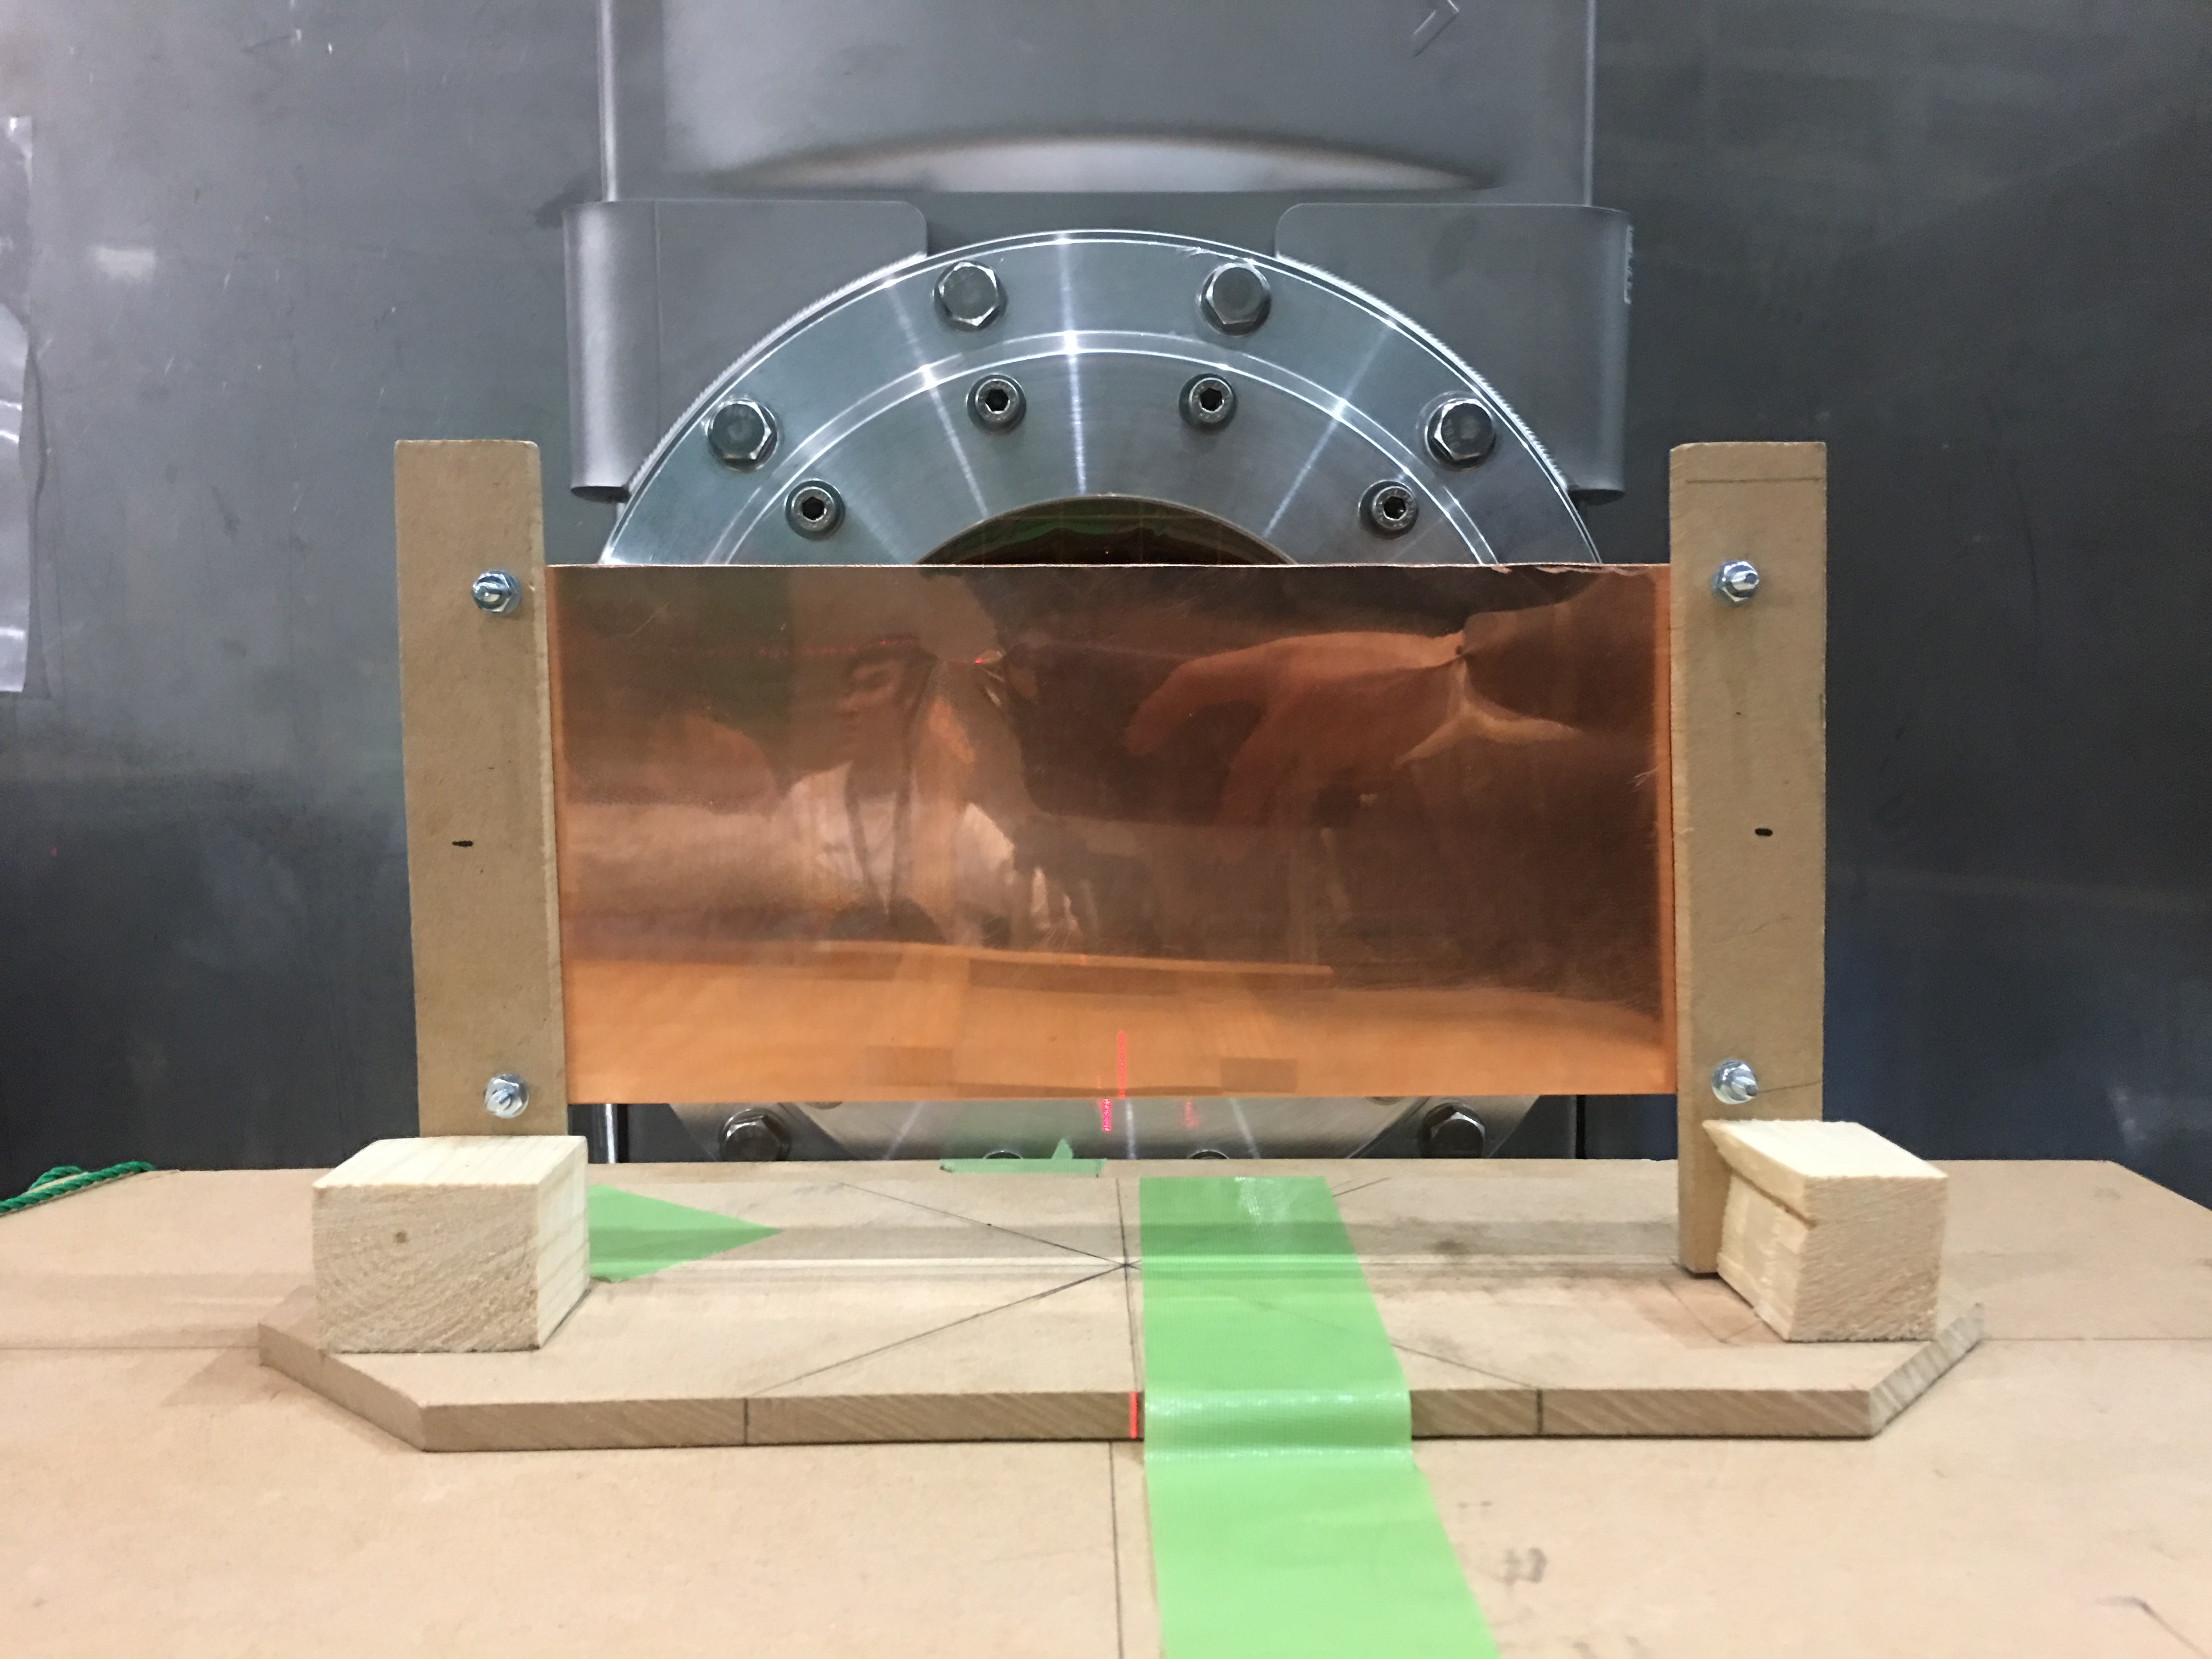
\includegraphics[width=1\textwidth]{figure/tajima/cu_target.jpg}
\caption{銅板標的}
\label{tar_cu}
\end{center}
\end{minipage}
\hfill
\begin{minipage}{0.45\hsize}
\begin{center}
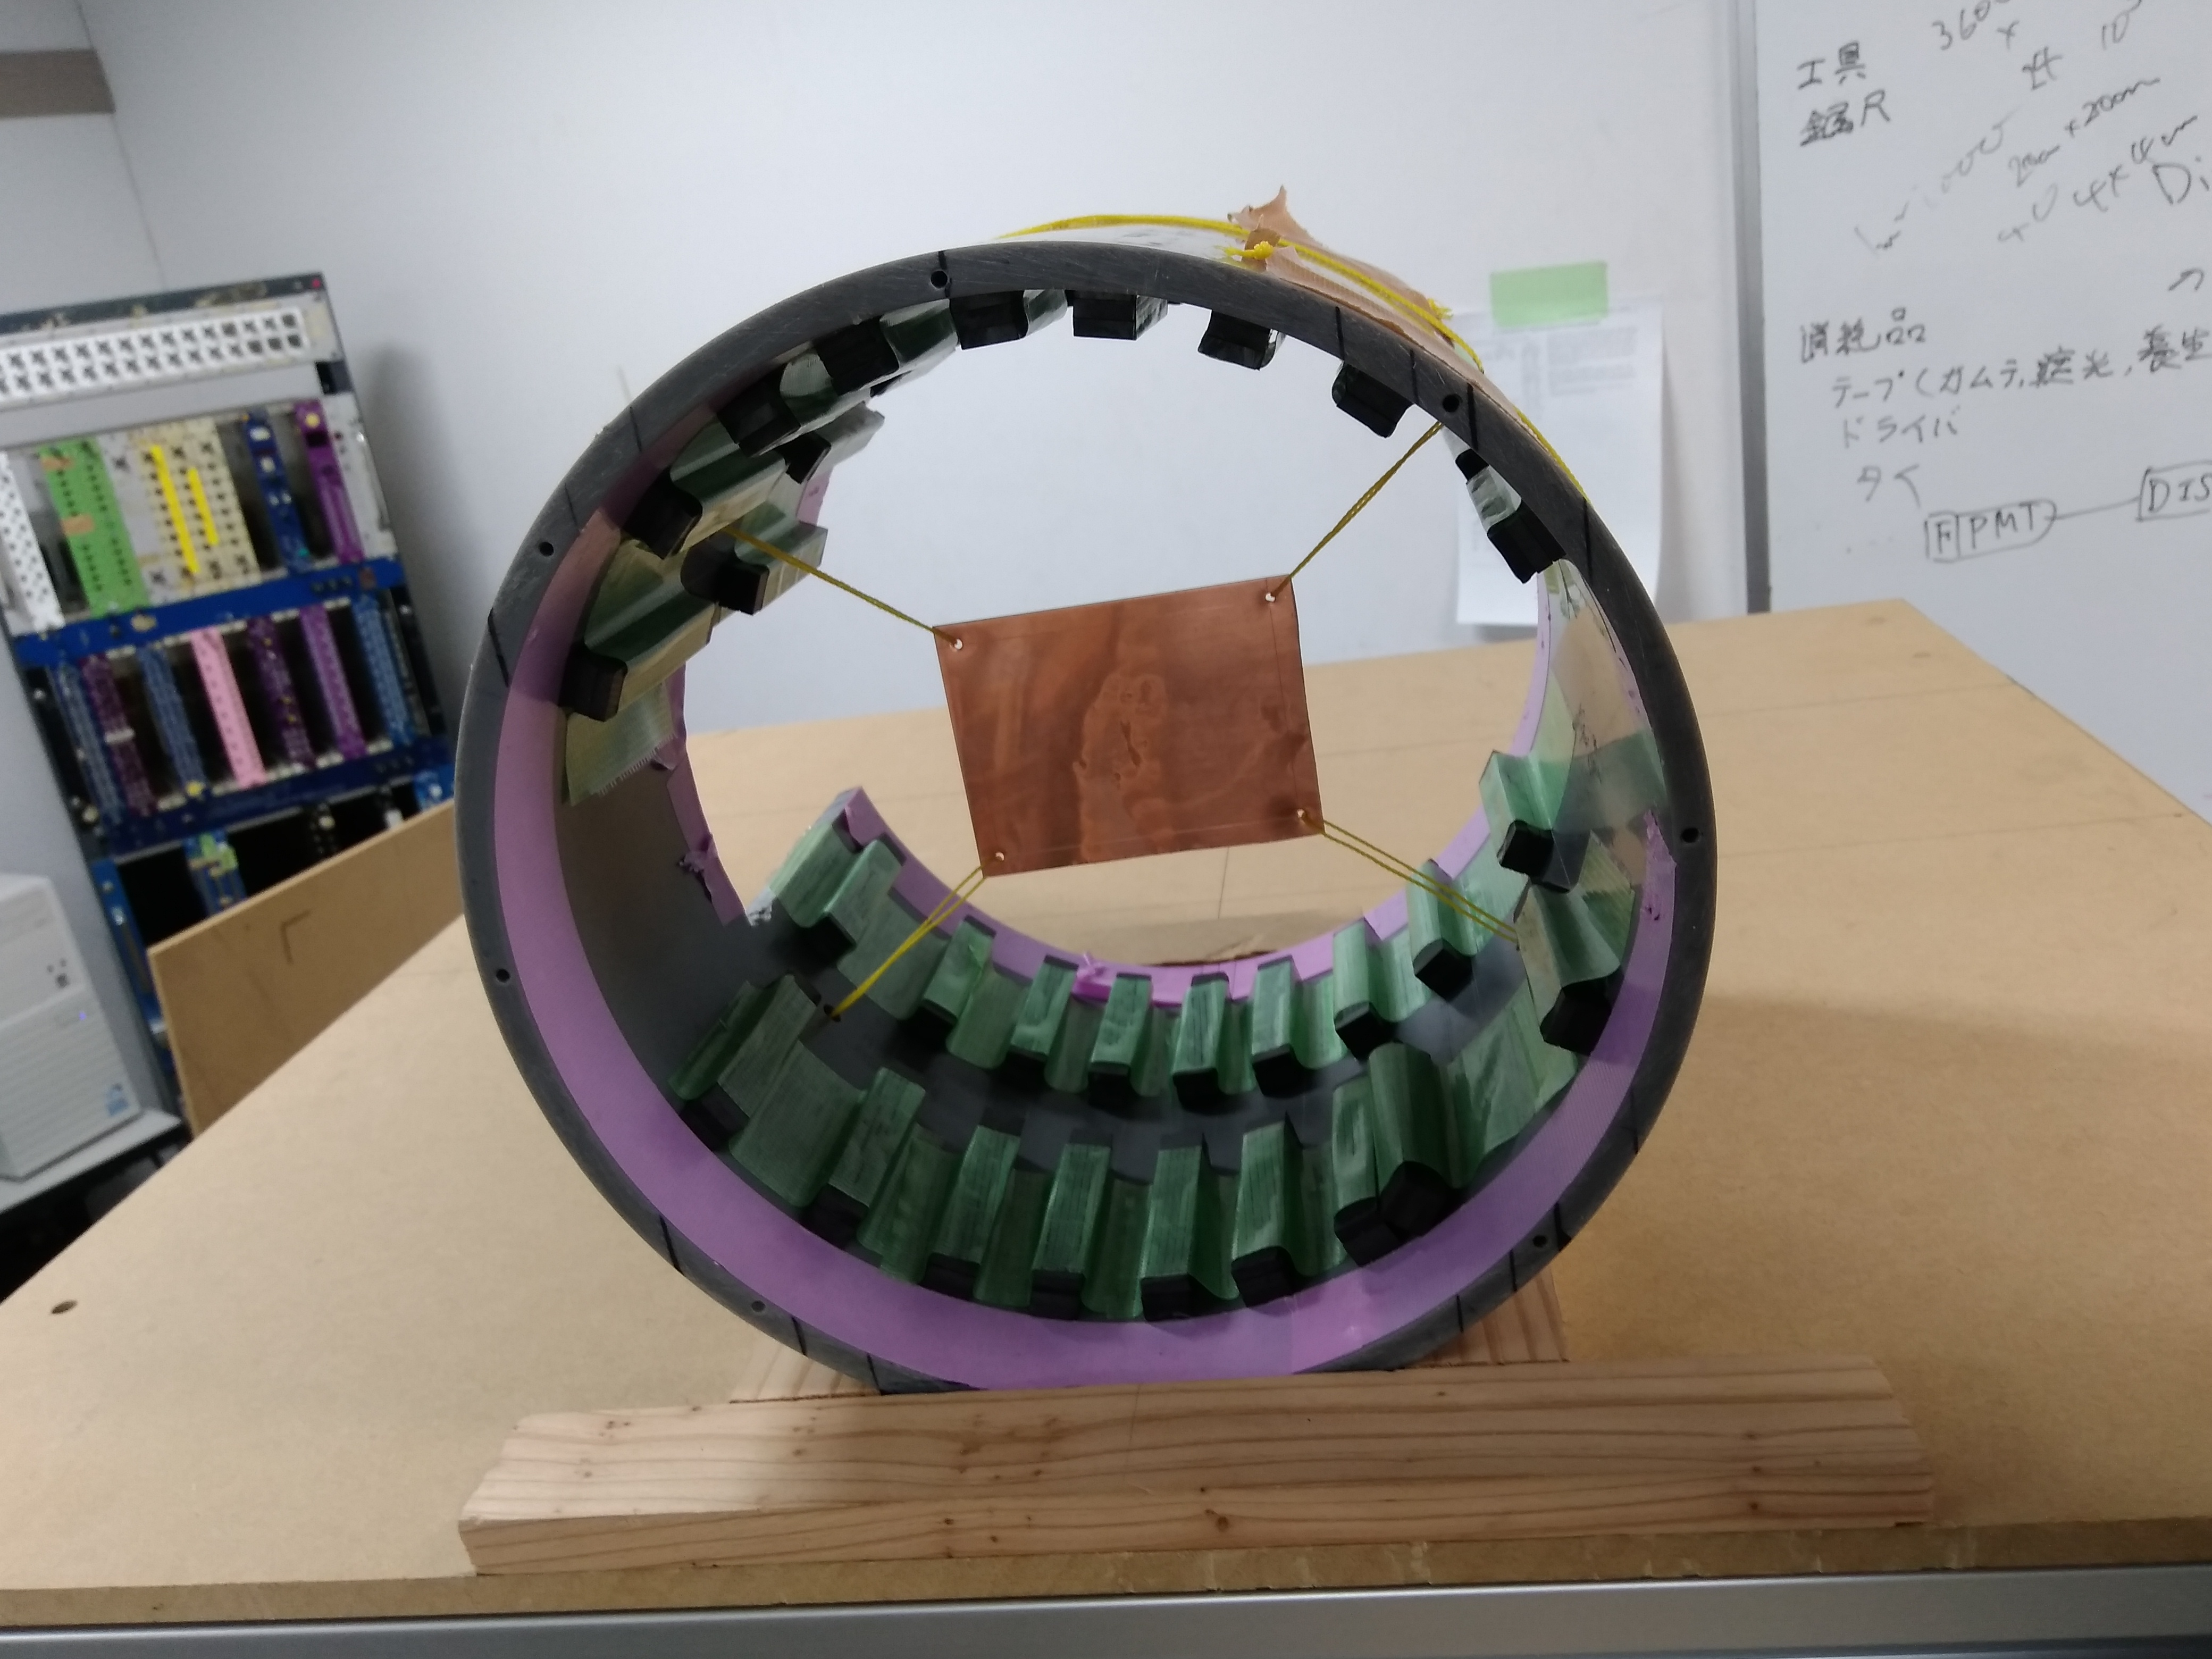
\includegraphics[width=1\textwidth]{figure/tajima/mag.jpg}
\caption{磁場発生装置と標的 \protect\footnotemark}
\label{tar_mag}
\end{center}
\end{minipage}
\end{figure}
\footnotetext{写真では下方の磁石が外れているが,これは実験前に修復した.}

\subsubsection{磁場の発生原理について: $\cos \theta$配置}
磁場の生成には$\cos n \theta$ 巻き ($n=1$) の電磁石を参考にした.$\cos n \theta$ 巻きの電磁石の考え方は以下のものである.図~\ref{cos2}, \ref{cos4} のように,十分長い円環上を電流が$z$ 軸方向に流れているとする.この電流密度が$\cos n\theta$ (ここで$\theta$ は円柱座標 ($r,\theta,z$) における$\theta$ のことで,$n$ は整数)に比例したとする.すると原点付近の領域に, $2n$ 極磁場が形成されるというものである.導出の概略は,円環各点が形成する磁場をその点の周りでテーラー展開し,これを$\theta$ について積分すると$2n$ 極磁場を形成する項のみが残るというものである.\cite{mag}

\begin{figure}[H]
\begin{minipage}{0.45\hsize}
\centering
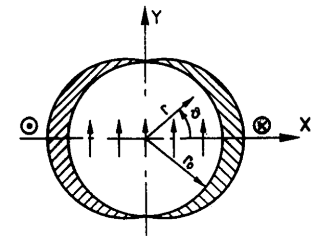
\includegraphics[width=0.8\textwidth]{figure/tajima/cos.png}
\caption{$\cos\theta$ : 2 極磁石\cite{magnet}}
\label{cos2}
\end{minipage}
\hfill
\begin{minipage}{0.45\hsize}
\centering
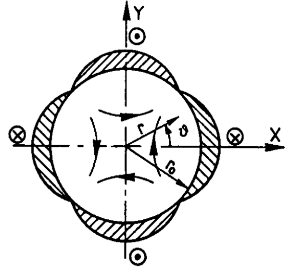
\includegraphics[width=0.7\textwidth]{figure/tajima/cos2.png}
\caption{$\cos 2 \theta$ : 4 極磁石\cite{magnet}}
\label{cos4}
\end{minipage}
\end{figure}

作成の手軽さから,磁場発生源には電磁石ではなく永久磁石(セラミック磁石)を用いた.電磁石における電流密度を,永久磁石の分布密度で置き換え,磁石の分布密度が$|\sin\theta|$ に比例するようにした.$\sin\theta$ としたのは磁石の向きをすべて動径方向に向けて配置すると,電磁石の場合に比べて磁場の向きが$\pi/2$ だけずれるためである.また各磁石の磁場方向は$0 < \theta < \pi$ と$\pi < \theta < 2\pi$ で動径方向に対して正と負になるようにした.

作成に入る前に,考えた配置をFEMM を用いてシミュレートし,磁場の一様性を確認した.図~\ref{femm}はFEMM によるシミュレーション結果で、赤線の太枠で囲われた領域が銅板に対応している。実際に有限の長さの磁石で磁場装置を作成するにあたって,図~\ref{tar_mag} のように磁石を長手方向に$3~\mathrm{cm}$ の間隔を開けて配置した.これは,間隔を開けることにより長手方向に隙間を空けずに磁石を詰めたときに比べて,磁力線が緩和され長手方向に磁場の一様性が増すと考えたためである.

\begin{figure}[H]
\centering
\includegraphics[width=0.9\textwidth]{figure/tajima/femm_modify1-1.pdf}
\caption{FEMMによる2次元シミュレーション}\label{femm}
\end{figure}


\newpage

\subsection{予備実験}

\subsubsection{プラスチックシンチレータの宇宙線較正}
プラスチックシンチレータでミューオンの崩壊から生じる陽電子のエネルギーを測定するために, 宇宙線を用いてエネルギー較正を行った.

%%%%%%挿入&修正by池満%%%%%%%%
ケーブル類とHV 値は本実験の状態と同様の状態にしたうえで,本実験において陽電子が入射する面を上にむけて宇宙線の測定を行った.各PMT にかけた電圧を表~\ref{PS_PMT_HV} に示す.データ取得の条件は,WFD のチャンネルトリガーを用いて全チャンネルのORでトリガーをとり,1 波形分を取れるような時間幅としてゲートは208~ns とした.このときのトリガーのしきい値は全チャンネルで共通にしており,電圧値は各チャンネルのレートが約$3 \sim 5~\mathrm{Hz}$になるように選んだ.
\begin{table}[H]
\caption{プラスチックシンチレータ用のPMT のHV 値}
\label{PS_PMT_HV}
\centering
\begin{tabular}{cc}\toprule
PMT 名 & HV値 \\ \midrule
チャンネル0(あけみ)& $-1600~\mathrm{V}$ \\
チャンネル1(勝太郎)& $-1418~\mathrm{V}$ \\
チャンネル2(畑さん)& $-1940~\mathrm{V}$ \\
チャンネル3(紗智子)& $-1762~\mathrm{V}$ \\
チャンネル4(蘭)  & $-1871~\mathrm{V}$ \\
チャンネル5(矢部) & $-1947~\mathrm{V}$ \\
チャンネル6(政子) & $-1980~\mathrm{V}$ \\
チャンネル7(王)  & $-1905~\mathrm{V}$ \\ \bottomrule
\end{tabular} 
 \end{table}%

得られたWFD の電圧信号を時間積分し,さらに抵抗値$50~\Omega$ で割ることで,
信号の電荷量~[pC] を得た.各チャンネル毎の電荷量のヒストグラムは図~\ref{cosmicray} のようになり,図中の3 つのピークの由来を左からそれぞれペデスタル,環境放射線,宇宙線と考えた.
\begin{figure}[H]
\centering
\includegraphics[height = 0.9\columnwidth , angle = -90]{figure/ikemitsu/cosmicray_modify.pdf}
\caption{宇宙線測定で得られた各チャンネルの電荷量のヒストグラム.横軸は信号の電荷量の積分値~[pC],縦軸はカウント数である. }
\label{cosmicray}
\end{figure}%

宇宙線によるピークの部分を,Landau 関数をガウシアンで畳み込み積分した関数(以下,Langauss 関数と呼ぶ.)でフィッテイングを行った.ガウシアンで畳み込み積分をしたのは,プラスチックシンチレータとPMT で測定されるエネルギーには比較的大きいゆらぎがあるからである.そしてフィッテイングにより得られた最頻値をエネルギー損失12~MeV に対応する電荷量とした.ただし,最頻値に対応するエネルギー損失の見積もりは次の2つの仮定を基にしている.
\begin{itemize}
\item 宇宙線ミューオンは最小電離粒子でありプラスチックシンチレータ中でのエネルギー損失は$dE/dx \sim 2~\mathrm{MeV/cm}$ である.
\item 最頻値をとるのは宇宙線がシンチレータの底面に対して垂直に入射したとき,すなわち1~層を通過する飛跡の長さが6~cm のときである.
\end{itemize}
この仮定から,1~層でのエネルギー損失の最頻値は$2~\mathrm{MeV/cm} \times 6~\mathrm{cm} = 12~\mathrm{MeV}$ に対応すると判断した\cite{leo}.
さらにペデスタルをガウシアンでフィットしてエネルギーの0点に対応する電荷を求めた.図~\ref{ps_langau} は各チャンネルの積分電荷の分布をLangauss 関数(赤線)でフィッティングしたものである.図~\ref{ps_cali} は宇宙線較正の結果を図にしたものである.黒色の誤差バー付きの点が較正点,赤色の直線が二点を基に引いた直線である.

\begin{figure}[H]
\centering
\includegraphics[height=0.7\textwidth,angle=-90]{figure/ikemitsu/fit_langau_modify.pdf}
\caption{Langauss 関数を用いた宇宙線ピークのフィッティング.横軸を信号の電荷量の積分値~[pC],縦軸をカウント数とした. }
\label{ps_langau}
\end{figure} 
\begin{figure}[H]
\centering
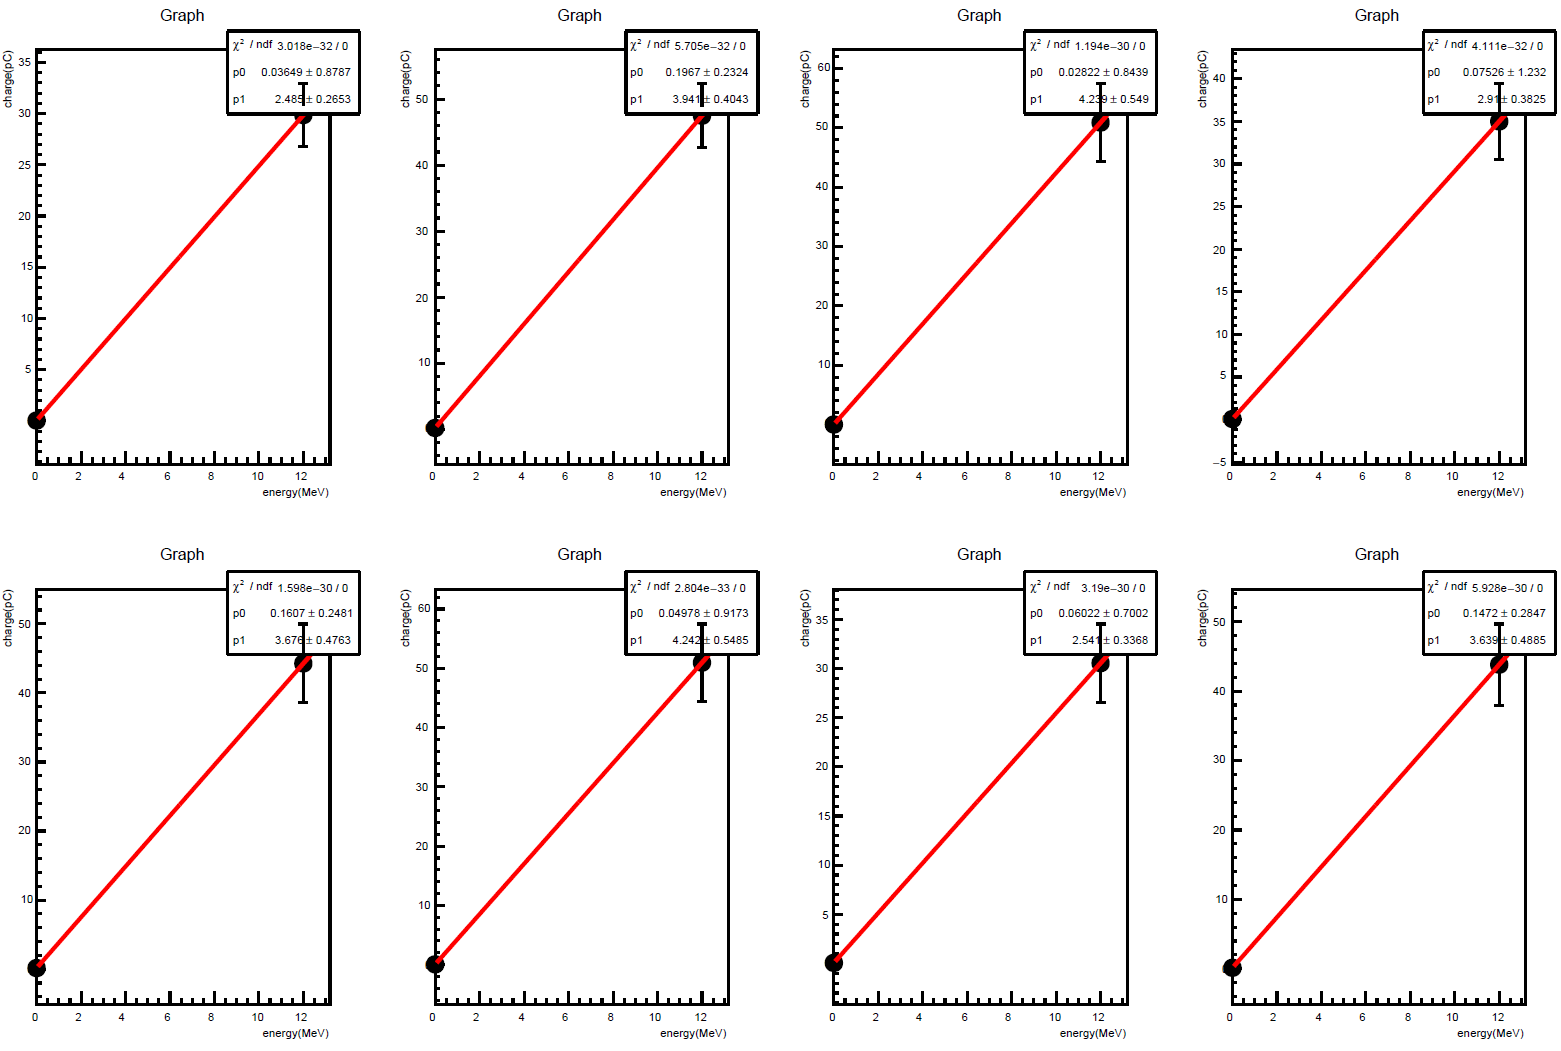
\includegraphics[height=0.9\textwidth,angle=-90]{figure/ikemitsu/fit_calibline.pdf}
\caption{プラスチックシンチレータの宇宙線較.横軸を粒子の損失エネルギー,縦軸を対応するエネルギーとした.ペデスタルと宇宙線の測定結果を基に直線を引くことでエネルギー較正を行った.}\label{ps_cali}
\end{figure}

較正の結果は表~\ref{PS_calib_table} のようになった.
表中の$a, b$ は,それぞれエネルギー$E~[\mathrm{MeV }]$ と電荷$Q~[\mathrm{pC}]$ の対応を$E = a Q + b$ としたときの定数である.
\begin{table}[h]
\caption{較正の結果}
\label{PS_calib_table}
\centering
\begin{tabular}{ccc}\toprule
チャンネル番号 & $a$ & $b$ \\ \midrule
0 & 0.40$\pm$0.040 & 0$\pm$0.30 \\
1 & 0.25$\pm$0.030 & 0$\pm$0.06 \\
2 & 0.24$\pm$0.030 & 0$\pm$0.20 \\
3 & 0.34$\pm$0.045 & 0$\pm$0.40 \\
4 & 0.27$\pm$0.035 & 0$\pm$0.07 \\
5 & 0.24$\pm$0.030 &0 $\pm$0.21 \\
6 & 0.39$\pm$0.050 &0 $\pm$0.30 \\
7 & 0.27$\pm$0.040 &0 $\pm$0.08 \\ \bottomrule
\end{tabular}
\end{table}%

\subsubsection{NaI のゲイン測定}
本実験で用いるNaI 検出器が出力する信号は,NaI の9 本とフィンガーカウンターの計10 個であった.一方でNaI の信号の処理に用いるWFD の入力できるチャンネル数は8 つであった.このため,WFD に入力する前にNaI からの信号をアナログの段階で足し合わせて信号の数を絞る必要があった.

各ch 間で,NaI 結晶自体の発光量も違い,NaI に付属するPMT のゲインもHV 値(PMT にかける高電圧)に対する依存性が個体毎に大きく異なる.一方で,足し合わせるNaI の信号の大きさは同じエネルギーに対して同じにしなければならかったため,それぞれのNaI のゲインカーブの測定を行った.この測定したゲインからどのようにNaI の信号を足し合わせるかを決めた.

まずNaI のゲインを測定するためにHV 値を変えながら線源${}^{137}\mathrm{Cs}$ を用いて,検出器用に用意した計11本のNaI (1 から順番に11 まで番号を付けた)の電荷の測定を行った(この線源は661.7keV のガンマ線を放出する)\cite{IAEA_ENSDF} .プラスチックシンチレータの宇宙線較正と同様にして,WFD からの電圧信号から電荷分布を得た.これを光電ピークと考えられるところでそれぞれガウシアンでフィッティングし,得られた平均値をゲインとした.さらにゲインについて以下の式が成り立つとし,両対数でフィッティングを行った\cite{Hamamatsu_PMT} .
\begin{equation}
\mathrm{Gain}~[\mathrm{pC}] = a \times \mathrm{HV}~[\mathrm{kV}]^b \label{gain_curve}  
\end{equation}
ただし$a, b$ はフィッティングパラメータである.その結果が図~\ref{GainHV} である.

また各HV 値でのエネルギー分解能とHV の関係が図~\ref{resoHV} である.ただし分解能はガウシアンの$\sigma$ を電荷で割ったものである.
\begin{figure}[H]
\begin{minipage}{0.45\hsize}
\centering
\hspace*{-1em}
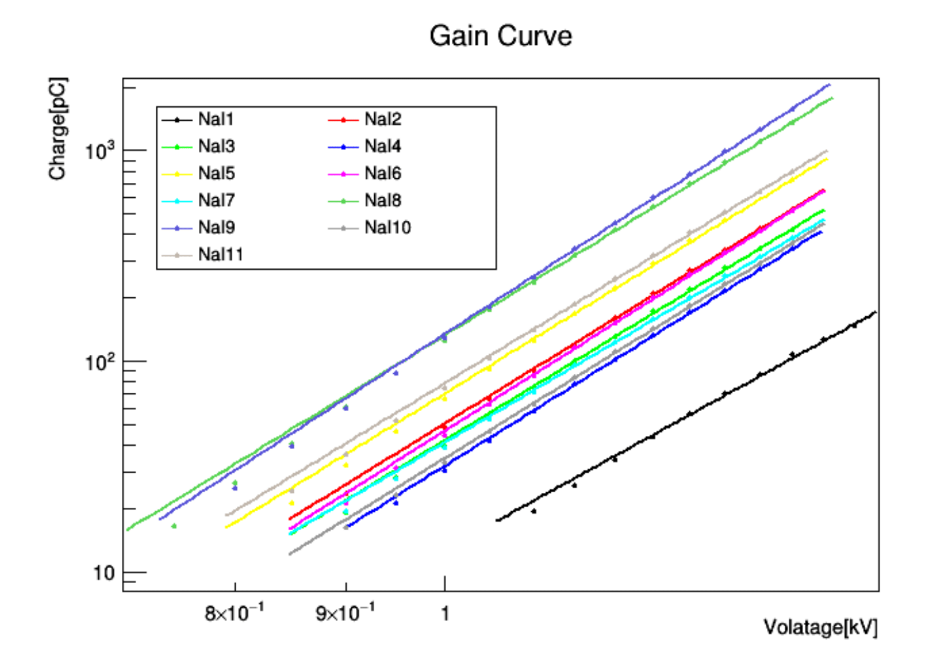
\includegraphics[width=1.1\textwidth]{figure/tajima/gain_curve.png}
\caption{ゲインとHV 値の対応.横軸をHV 値~[kV],縦軸をゲインに相当する電荷量~[pC]とした.}
\label{GainHV}
\end{minipage}
\hfill
\begin{minipage}{0.45\hsize}
\centering
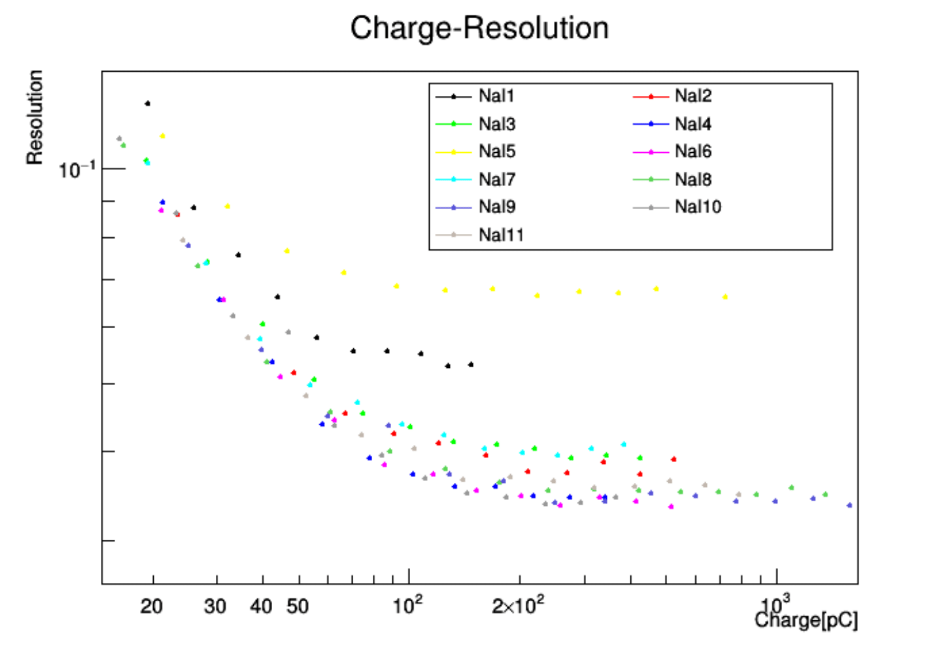
\includegraphics[width=1.1\textwidth]{figure/tajima/charge_resolution.png}
\caption{ゲインと分解能の対応.横軸を分解能,縦軸をゲイン~[pC]1とした.}
\label{resoHV}
\end{minipage}
\end{figure}
この結果, NaI1 はゲインが低く,NaI5 に関しては分解能が悪かったため,本実験では用いないことにした(以降,NaI1,5 で測定を行わないことにした).
またNaI10 は分解能が良かったため,足し合わせず中心に配置するNaI とした.

上の結果を用いて,ゲインの調整を行った.上のゲインに$50~\mathrm{MeV} /661.7~\mathrm{keV}$ をかけて,スケール変換することで得られた曲線を$50~\mathrm{MeV}$ におけるゲイン曲線とした.そして最大エネルギー$\sim 50~\mathrm{MeV}$ の入力信号の波高~[V] がWFD の入力電圧の上限の半分である$1~\mathrm{V}$ ($500~\mathrm{pC}$) になるように設定した.

表~\ref{HV} が各HV 値の調整値を表にしたものである.ここで入力信号の電圧と電荷の関係は以下のように求めた.まずNaI の波形は立ち上がり時間にくらべ立ち下がり時間が長いので,立ち上がりがステップ関数で立ち下がりが指数関数であることを近似的に仮定した.この時にNaI の信号の減衰時間幅は約$T \sim 250~\mathrm{ns}$ なので,最大電圧$V_\mathrm{max}~[\mathrm{V}]$ の信号電荷は以下のように概算できる.
\begin{equation}
Q~[\mathrm{C}] = \frac{V_\mathrm{max}~[\mathrm{V}] \times T~[\mathrm{s}]}{R~[\Omega]}
\end{equation}
ここで$R$ はWFD の抵抗値で$50~\Omega$ である.

今回測定に用いた線源のエネルギーは661.7~keV であるのに対して,実際の測定の最大エネルギーは約50~MeV であり,線源のエネルギーに比べてかなり大きかった.よって高いエネルギー領域においても上のゲイン曲線が成り立っていることの確認を行った.そのために,表~\ref{HV} のHV 値で宇宙線の測定を行った.そして,得られた電荷分布をLangauss 関数でフィッテイングを行い,得られた最頻値をゲインとすると,表~\ref{nai_gain} のようになった.

このゲインの値が近く,また分解能の値が近いものを足し合わせるペアとし,これを(2,7),(3,9),(4,6),(8,11)の4組に決めた.これらのペアの宇宙線におけるゲインのずれはいずれも10~\%程度となった.

\begin{table}[H]
\begin{minipage}[t]{0.45\textwidth}
\centering
\caption{NaI のHV 設定}\label{HV}
\begin{tabular}{cc}\toprule
NaI No. & HV~[V]\\ \midrule
2 & 1050 \\
3 & 1082 \\
4 & 1125 \\
6 & 1062 \\
7 & 1089 \\
8 & 913 \\
9 & 913 \\ 
10 & 1112 \\
11 & 984 \\ \bottomrule
\end{tabular}
\end{minipage}
\hfill
\begin{minipage}[t]{0.45\textwidth}
\centering
\caption{宇宙線の測定結果}\label{nai_gain}
\begin{tabular}{cc}\toprule
NaI No. & Gain~[pC]\\ \midrule
2 & 2530 \\
3 & 2387 \\
4 & 2352 \\
6 & 2397 \\
7 & 2579 \\
8 & 2423 \\
9 & 2164 \\
11 &2393 \\ \bottomrule
\end{tabular}
\end{minipage}
\end{table}

さらに本実験におけるNaI の配置を表~\ref{haichi} のように決めた.配置を決めるにあたって,以下の事柄を考慮した.
\begin{itemize}
\item エネルギー重心を求める観点からペアを中心から等距離になるように配置した.
\item 中心にフィンガーカウンターを置きコインシデンスをとることで,陽電子が中心のNaI に入射したときのみ測定することにし.このため中心のNaI で測定されるエネルギーは大きくなることが考えられるので,ゲインが低いものを中心に配置した.
\item 本実験のセットアップにおける宇宙線較正を想定した場合(実際には時間の都合上行っていない),測定データから宇宙線がどのNaI にヒットしたか区別できる必要があった.宇宙線は上方から飛来する可能性が高いとして,測定データからどのNaI に宇宙線がヒットしたかを判別できるように配置した.
\end{itemize}
\begin{table}[H]
\centering
\caption{ビーム正面からみたNaI の配置図}\label{haichi}
\begin{tabular}{|c|c|c|}\hline
\cellcolor{yellow}~3~ & \cellcolor{red}2 & \cellcolor{yellow}9\\ \hline
\cellcolor{cyan}~4~ & 10 & \cellcolor{red}7\\ \hline
\cellcolor{green}~8~ & \cellcolor{cyan}6 & \cellcolor{green}11\\ \hline
\end{tabular}
\end{table}

\newpage

\subsubsection{NaI の宇宙線較正}
NaI でエネルギーを測定するために, 宇宙線を用いてエネルギー較正を行った.
先にもとめたHV値のもとで,それぞれのNaI で宇宙線を測定した.
各NaI の上方と下方にプラスチックシンチレータを配置してコインシデンスをとることで,
貫通イベントのみを記録した.
またプラスチックシンチレータの位置をずらすと,測定される宇宙線のNaI 中での飛跡は長くなる.
この時の宇宙線は最小電離粒子とみなせるので,飛跡とエネルギーは比例する.
よって,プラスチックシンチレータの位置をすらすことで計3点のエネルギーを測定した.
そして,得られた電荷分布を,Langauss 関数でフィッテイングを行った.
図~\ref{langau} はあるセットアップにおける宇宙線測定のヒストグラムで,
赤線はLangauss 関数によるフィッテイング曲線である.

次にGeant4 を用いて,同じセットアップで宇宙線モンテカルロシミュレーションを行った.
図~\ref{MC2} はシミュレーションによるエネルギー分布である.
モンテカルロシミュレーションによって得られた最頻値と測定によって得られた最頻値でエネルギー較正を行った.

\begin{figure}[H]
\begin{minipage}{0.45\hsize}
\centering
\hspace*{-1em}
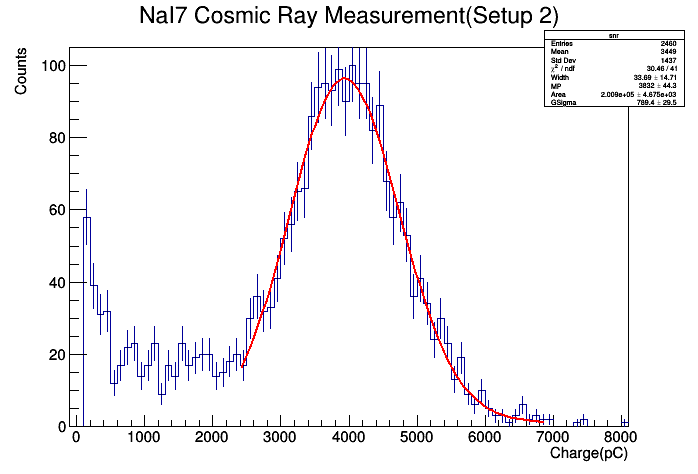
\includegraphics[width=1\textwidth]{figure/tajima/NaI7_Setup2.png}
\caption{あるセットアップにおける宇宙線測定の結果をLangauss 関数でフィッテイングしたもの.横軸を電荷量~[pC],縦軸をカウント数とした.}\label{langau}
\end{minipage}\hfill
\begin{minipage}{0.45\hsize}
\centering
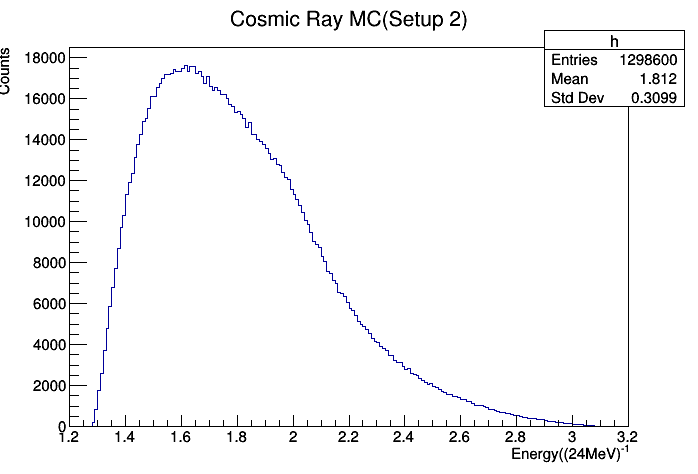
\includegraphics[width=1\textwidth]{figure/tajima/MC2.png}
\caption{左と同様のセットアップでシミュレーションを行って得られた宇宙線のエネルギースペクトル.横軸をエネルギーを24~MeVで規格化したもの,縦軸をカウント数とした.}\label{MC2}
\end{minipage}
\end{figure}

図~\ref{cali} は宇宙線較正の結果を図にしたものである.
\begin{figure}[H]
\centering
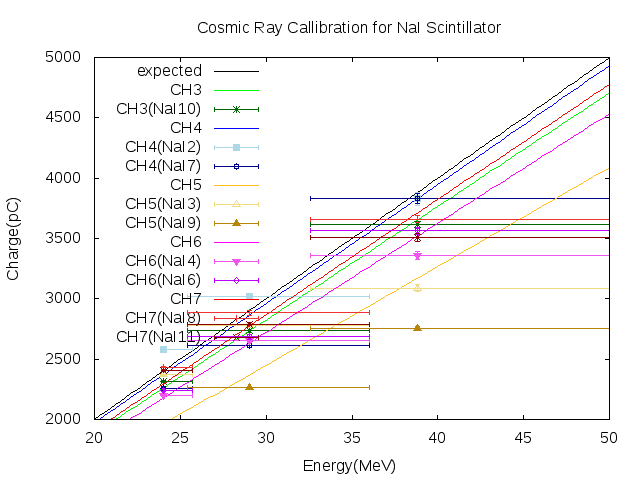
\includegraphics[width=0.7\textwidth]{figure/tajima/fit.eps}
\caption{各ch における宇宙線測定の電荷とエネルギーの対応関係.横軸をエネルギー~[MeV],縦軸をWFD で測定された電荷~[pC]とした.各セットアップにおける測定とシミュレーションの結果を基にした点に対して直線フィッテイングを行った.}\label{cali}
\end{figure}

\newpage

\subsubsection{磁場測定}
$g$ 因子測定のための磁場装置の測定を3 軸テスラメータで行った.銅板を置く範囲を,10~mm 間隔で計63 点測定した.本実験の測定中に磁石が外れてしまったので,磁石が外れる前後のデータとして実験前と実験後に測定した.

測定した結果を以下の表~\ref{MF1}, \ref{MF2} と図~\ref{mag1},\ref{vec1},\ref{mag2},\ref{vec2} に記す.$x, y$の単位は~[mm] で,磁場の単位は~[Gauss] である.原点を銅板の中心とし, $y, z$軸を鉛直方向上向きとビーム方向にとった.
\begin{table}[H]
\centering
\caption{各点の磁場の強さ(磁石が外れる前)}\label{MF1}
\begin{tabular}{|c||c|c|c|c|c|c|c|c|c|}\hline
$y \backslash x$ & -4 & -3 & -2 & -1 & 0 & 1 & 2 & 3 & 4 \\ \hline \hline
3 & 51.48 & 54.98 & 55.33 & 55.55 & 55.42 & 54.77 & 54.44 & 53.27 & 51.75 \\ \hline
2 & 56.25 & 56.78 & 56.87 & 56.84 & 56.41 & 56.16 & 55.93 & 55.71 & 55.35 \\ \hline
1 & 57.15 & 57.50 & 57.39 & 57.11 & 56.72 & 56.53 & 56.48 & 56.50 & 56.44 \\ \hline
0 & 57.60 & 57.49 & 57.19 & 56.72 & 56.54 & 56.48 & 56.53 & 56.58 & 55.98 \\ \hline
-1 & 56.66 & 56.78 & 56.66 & 56.48 & 56.39 & 56.34 & 56.35 & 56.31 & 56.12 \\ \hline
-2 & 53.45 & 54.74 & 55.29 & 55.54 & 55.60 & 55.60 & 55.53 & 55.14 & 54.3 \\ \hline
-3 & 50.62 & 51.95 & 53.45 & 53.93 & 54.20 & 54.20 & 54.05 & 53.11 & 51.25 \\ \hline
\end{tabular}
\end{table}
\begin{figure}[H]
\begin{minipage}{0.45\hsize}
\centering
\includegraphics[width=1\textwidth]{figure/tajima/mag1.eps}
\caption{磁場の強さの分布図(磁石が外れる前).横軸をx,縦軸をyとした.黒線に囲われた領域が銅板領域である.}
\label{mag1}
\end{minipage}
\begin{minipage}{0.45\hsize}
\centering
\includegraphics[width=1\textwidth]{figure/tajima/vec1.eps}
\caption{xy平面における磁場ベクトル(磁石が外れた後).横軸をx,縦軸をyとした.背面の色はz軸方向の磁場の大きさを表し,矢印の長さは磁場ベクトルの大きさに対応している.}
\label{vec1}
\end{minipage}
\end{figure}



\begin{table}[H]
\centering
\caption{各点の磁場の強さ(磁石が外れた後)}\label{MF2}
\begin{tabular}{|c||c|c|c|c|c|c|c|c|c|}\hline
$y \backslash x$ & -4 & -3 & -2 & -1 & 0 & 1 & 2 & 3 & 4 \\ \hline \hline
3 & 55.41 & 55.93 & 55.79 & 54.78 & 53.30 & 50.73 & 46.89 & 46.34 & 41.95 \\ \hline
2 & 57.25 & 57.06 & 56.28 & 54.92 & 53.77 & 52.01 & 49.83 & 48.45 & 48.44 \\ \hline
1 & 57.72 & 57.30 & 56.52 & 55.61 & 54.34 & 52.97 & 51.84 & 51.08 & 50.49 \\ \hline
0 & 57.55 & 56.94 & 56.30 & 55.54 & 54.61 & 53.67 & 52.98 & 52.40 & 52.34 \\ \hline
-1 & 57.00 & 56.57 & 55.94 & 55.24 & 54.58 & 53.99 & 53.45 & 53.05 & 52.73 \\ \hline
-2 & 55.48 & 55.37 & 55.04 & 54.64 & 54.30 & 53.83 & 53.39 & 52.53 & 51.81 \\ \hline
-3 & 52.23 & 53.03 & 53.28 & 53.29 & 53.18 & 52.71 & 52.00 & 51.51 & 50.12 \\ \hline
\end{tabular}
\end{table}
\begin{figure}[H]
\begin{minipage}{0.45\hsize}
\centering
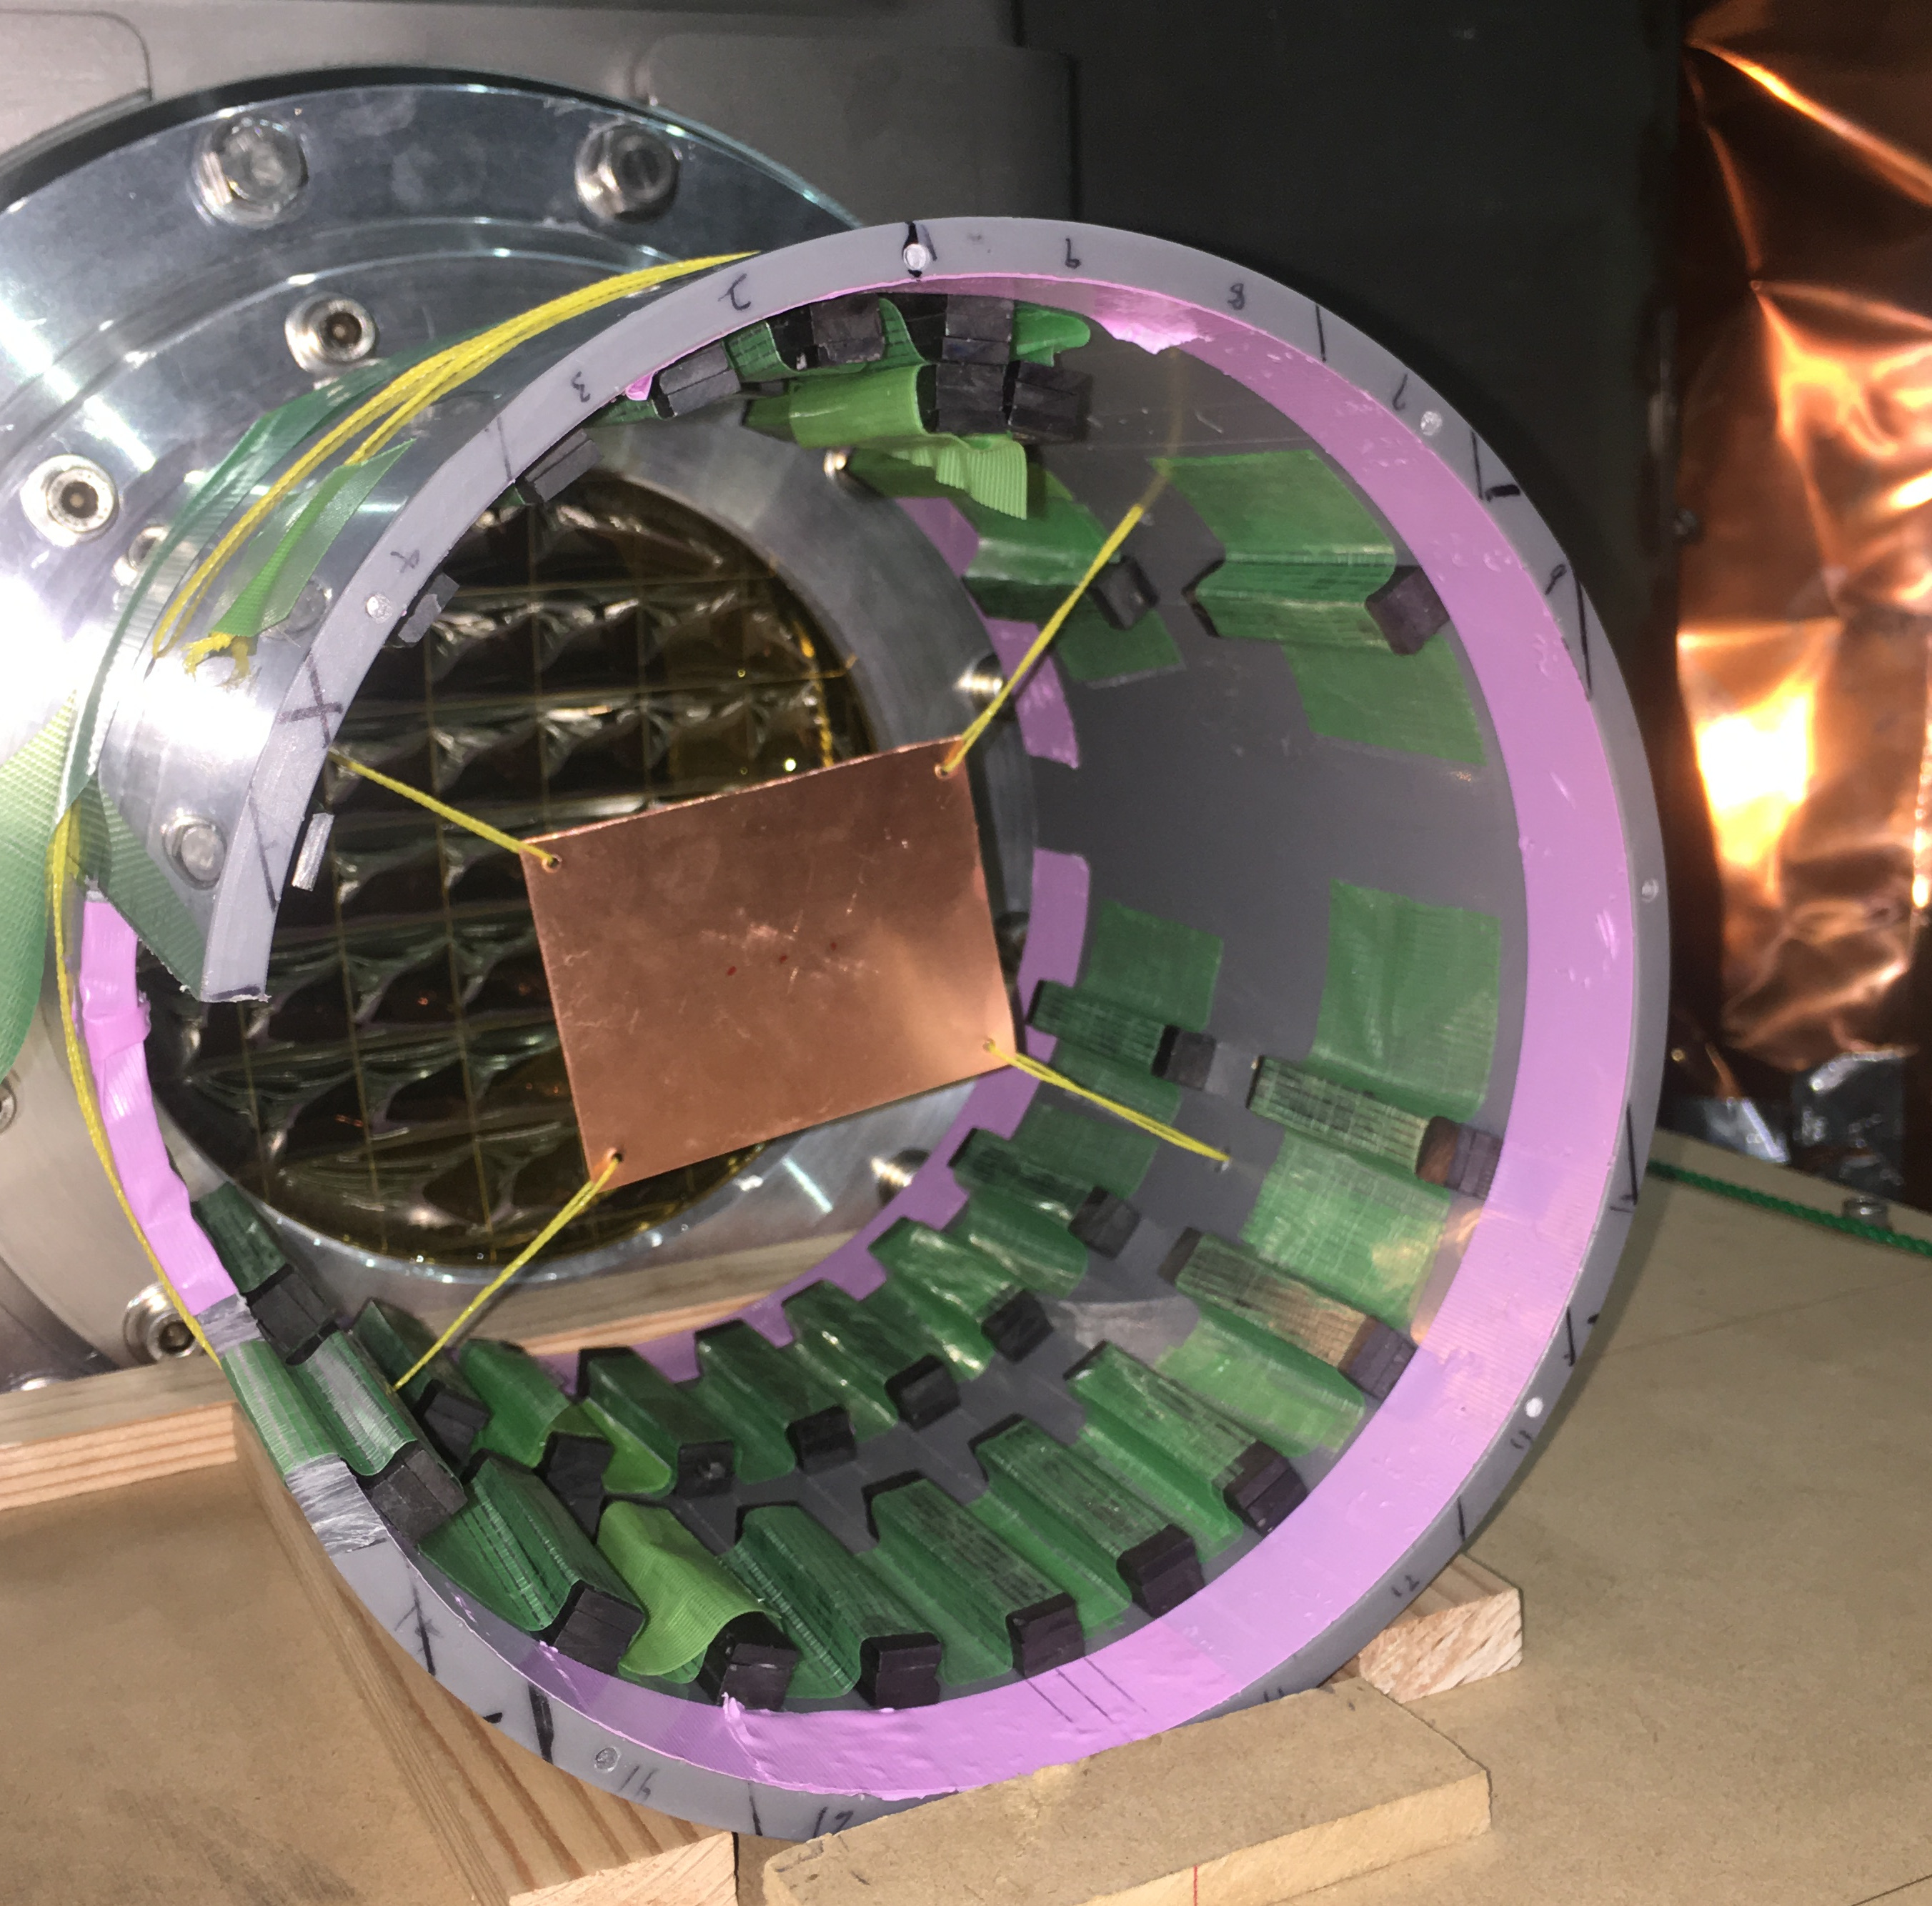
\includegraphics[width=1\textwidth]{figure/tajima/mag2.eps}
\caption{磁場の強さの分布図(磁石が外れた後).黒線に囲われた領域が銅板領域である.左手奥の磁石が外れ,隣の磁石についてしまった.これにより左部に磁場の偏りがみられる.}
\label{mag2}
\end{minipage}
\begin{minipage}{0.45\hsize}
\centering
\includegraphics[width=1\textwidth]{figure/tajima/vec2.eps}
\caption{xy平面における磁場ベクトル(磁石が外れた後).背面の色はz軸方向の磁場の大きさを表し,矢印の長さは磁場ベクトルの大きさに対応している.}
\label{vec2}
\end{minipage}
\end{figure}

$g$ 因子の計算に用いる磁場を得るために,予め頂いたビームプロファイルのデータ($\sigma_x = 33.3037~\mathrm{mm}, \; \sigma_y = 19.6668~\mathrm{mm}$) を用いて加重平均をとった.下図~\ref{beam_mag.eps}が加重平均に用いた重み分布で,平均$(\mu_x,\mu_y)=(0,0)$ ,分散$\sigma_x^2, \sigma_y^2$の2次元のガウシアンを規格化したものである.加重平均の結果,磁石が外れる前後の磁場がそれぞれ$56.06 \pm 1.20~\mathrm{G}$ と$53.97\pm 2.36~\mathrm{G}$ と求まった.誤差は統計誤差で,各点の測定の測定誤差を伝播させることで求めた.(系統誤差については後述.)

\begin{figure}[H]
\centering
\includegraphics[width=0.5\textwidth]{figure/tajima/beam_mag.eps}
\caption{加重平均に用いたビームプロファイル.黒線に囲われた領域が銅板領域である.}
\label{beam_mag}
\end{figure}

\newpage

\subsection{ビームを用いた本実験}

\subsubsection{タイムスケジュール}
本実験におけるスケジュールは以下の通りである.
\begin{itemize}
\item 2/25 (Sun.)\\
13:00   東海村到着,前日準備
\item 2/26 (Mon.) - 2/27 (Tue.)\\
9:00 - ロシアグループ $g - 2$ Beam Profile Monitor の実験の傍らで寿命を測定,セットアップの確認, 磁場測定(磁石が外れる前)
\item 2/28 (Wed.)\\
12:30  \phantom{-} ロシアグループの実験終了,銅板標的にて実験開始\\ 
12:30 - 21:30 セットアップの確認\\
21:47 - 24:00 磁場ターゲットを置いて,$g$ 因子をNaI のみで測定\\
24:20 - 29:50 磁場ターゲットを置いて,$g$ 因子をPS を加えて測定(測定の途中で磁石が外れる)
\item 3/1(Thu.)\\
7:20 \phantom{-} 磁場測定(磁石が外れた後)\\
7:20 - 8:10 銅板標的を置いて,エネルギーと寿命を測定\\
8:30 \phantom{-} ビームタイム終了\\
8:30 - 14:30 実験装置の放射線チェック及び後片付け \\
14:30 帰宅
\end{itemize}

\subsubsection{セットアップ}
この節では本実験のセットアップについて記す.まず寿命測定のセットアップは図~\ref{set_life}, \ref{set_life2} のようであった.図~\ref{set_life} が上からみたセットアップ図で図~\ref{set_life2} が実際のセットアップの写真である.ここでFC ,PS はフィンガーカウンターとプラスチックシンチレータの略で,Target は先に述べた銅板標的のことである.標的から測定器までの距離をビーム1~pulse あたりの陽電子のカウント数から決定した.

今回の測定では解析の都合から,陽電子がNaI では1~pulse あたり5 - 6 個に,プラスチックシンチレータでは8 - 9 個になるように調整を行った.その結果,標的からNaI ,プラスチックシンチレータまでの距離はそれぞれ$115~\mathrm{cm}, \; 75~\mathrm{cm}$ ,標的の中心からNaI ,プラスチックシンチレータまでの直線とビーム方向のなす角はそれぞれ$41^{\circ}, \;  47^{\circ}$ となった.
また標的とビーム窓の距離は17~cm であった.
\begin{figure}[H]
\begin{minipage}{0.45\hsize}
\centering
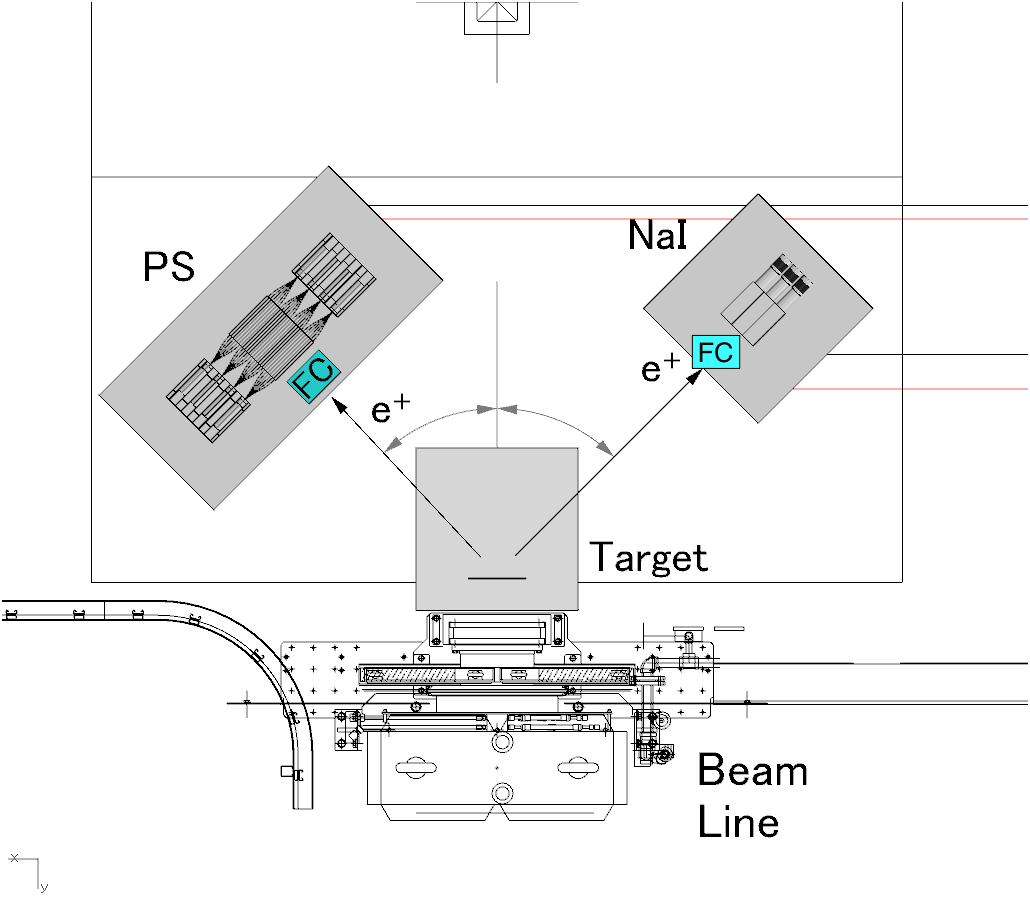
\includegraphics[width=1\textwidth]{figure/tajima/set_lifetime.png}
\caption{寿命測定のセットアップ}
\label{set_life}
\end{minipage}
\begin{minipage}{0.45\hsize}
\centering
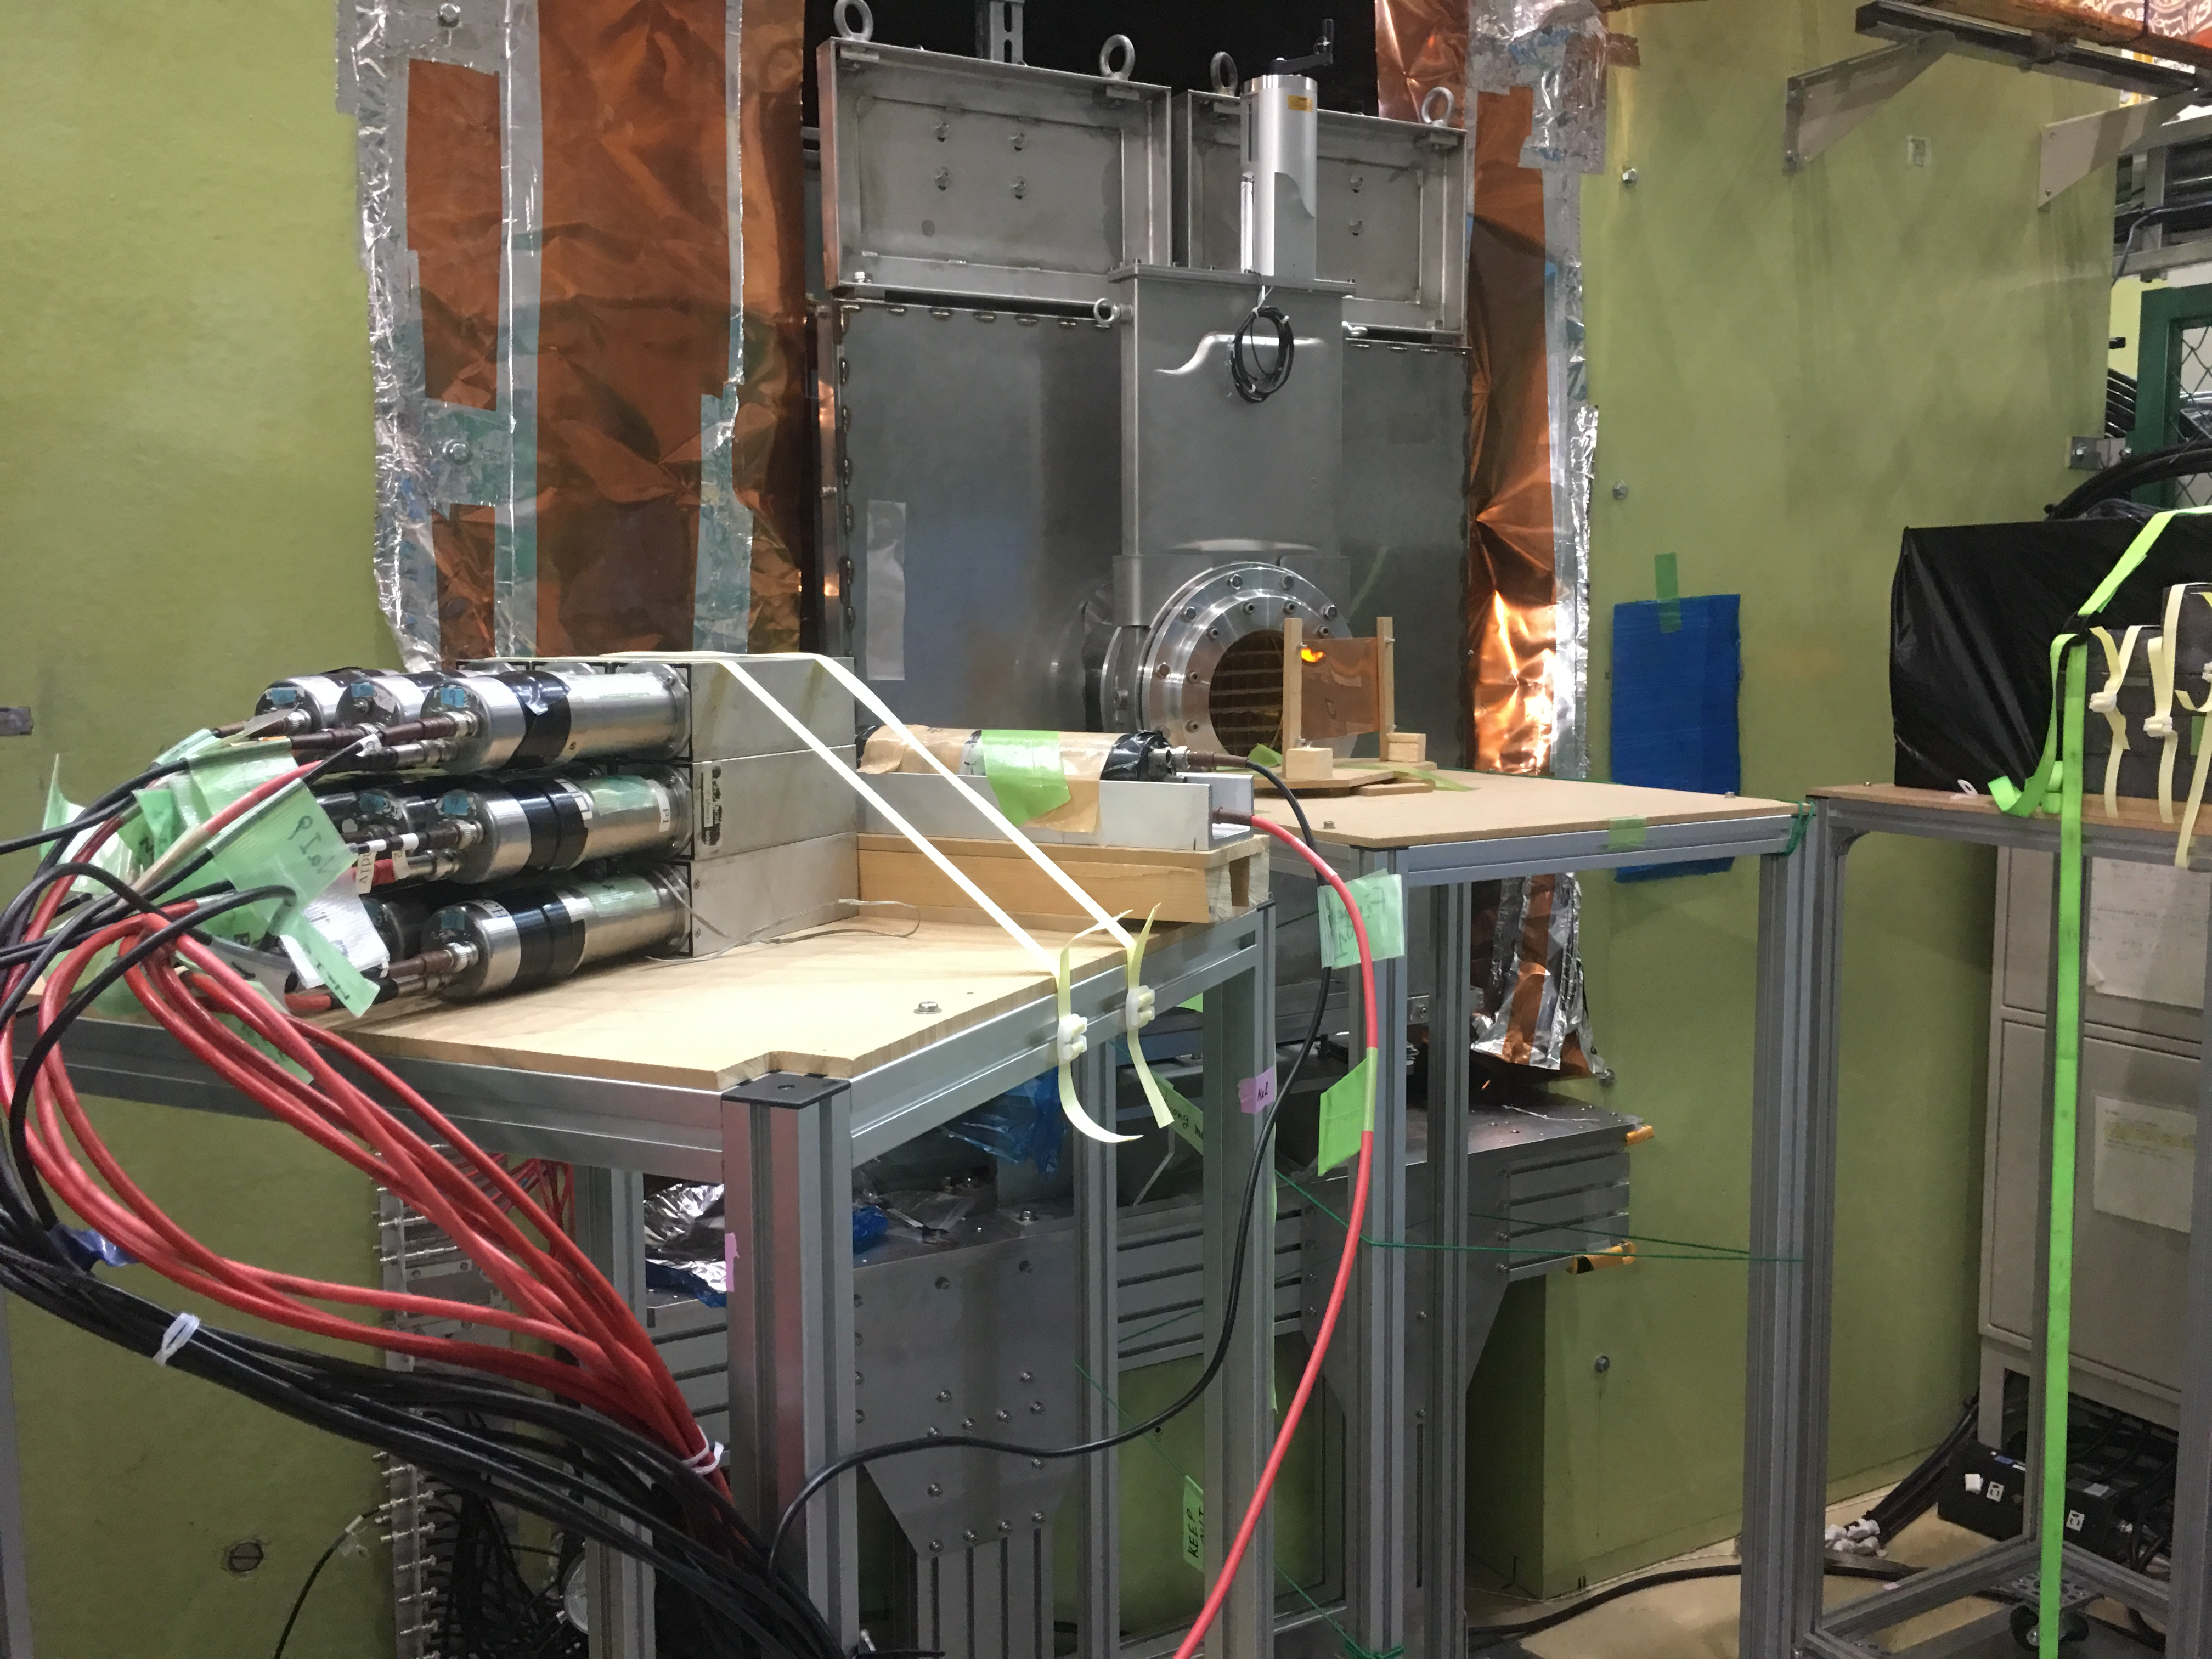
\includegraphics[width=1\textwidth]{figure/tajima/set_lifetime_1.png}
\caption{寿命測定のセットアップ(写真)}
\label{set_life2}
\end{minipage}
\end{figure}

次にエネルギー,$g$ 因子測定のセットアップについて示す.図~\ref{set_life} が上空からみたセットアップ図で,図~\ref{set_g_2} が実際のセットアップの写真である.ここでTarget には先に記した磁場印加標的を用いた.また検出器と標的の距離やビーム軸と標的から検出器のなす角は寿命測定と同じ値になるようにした.
\begin{figure}[H]
\centering
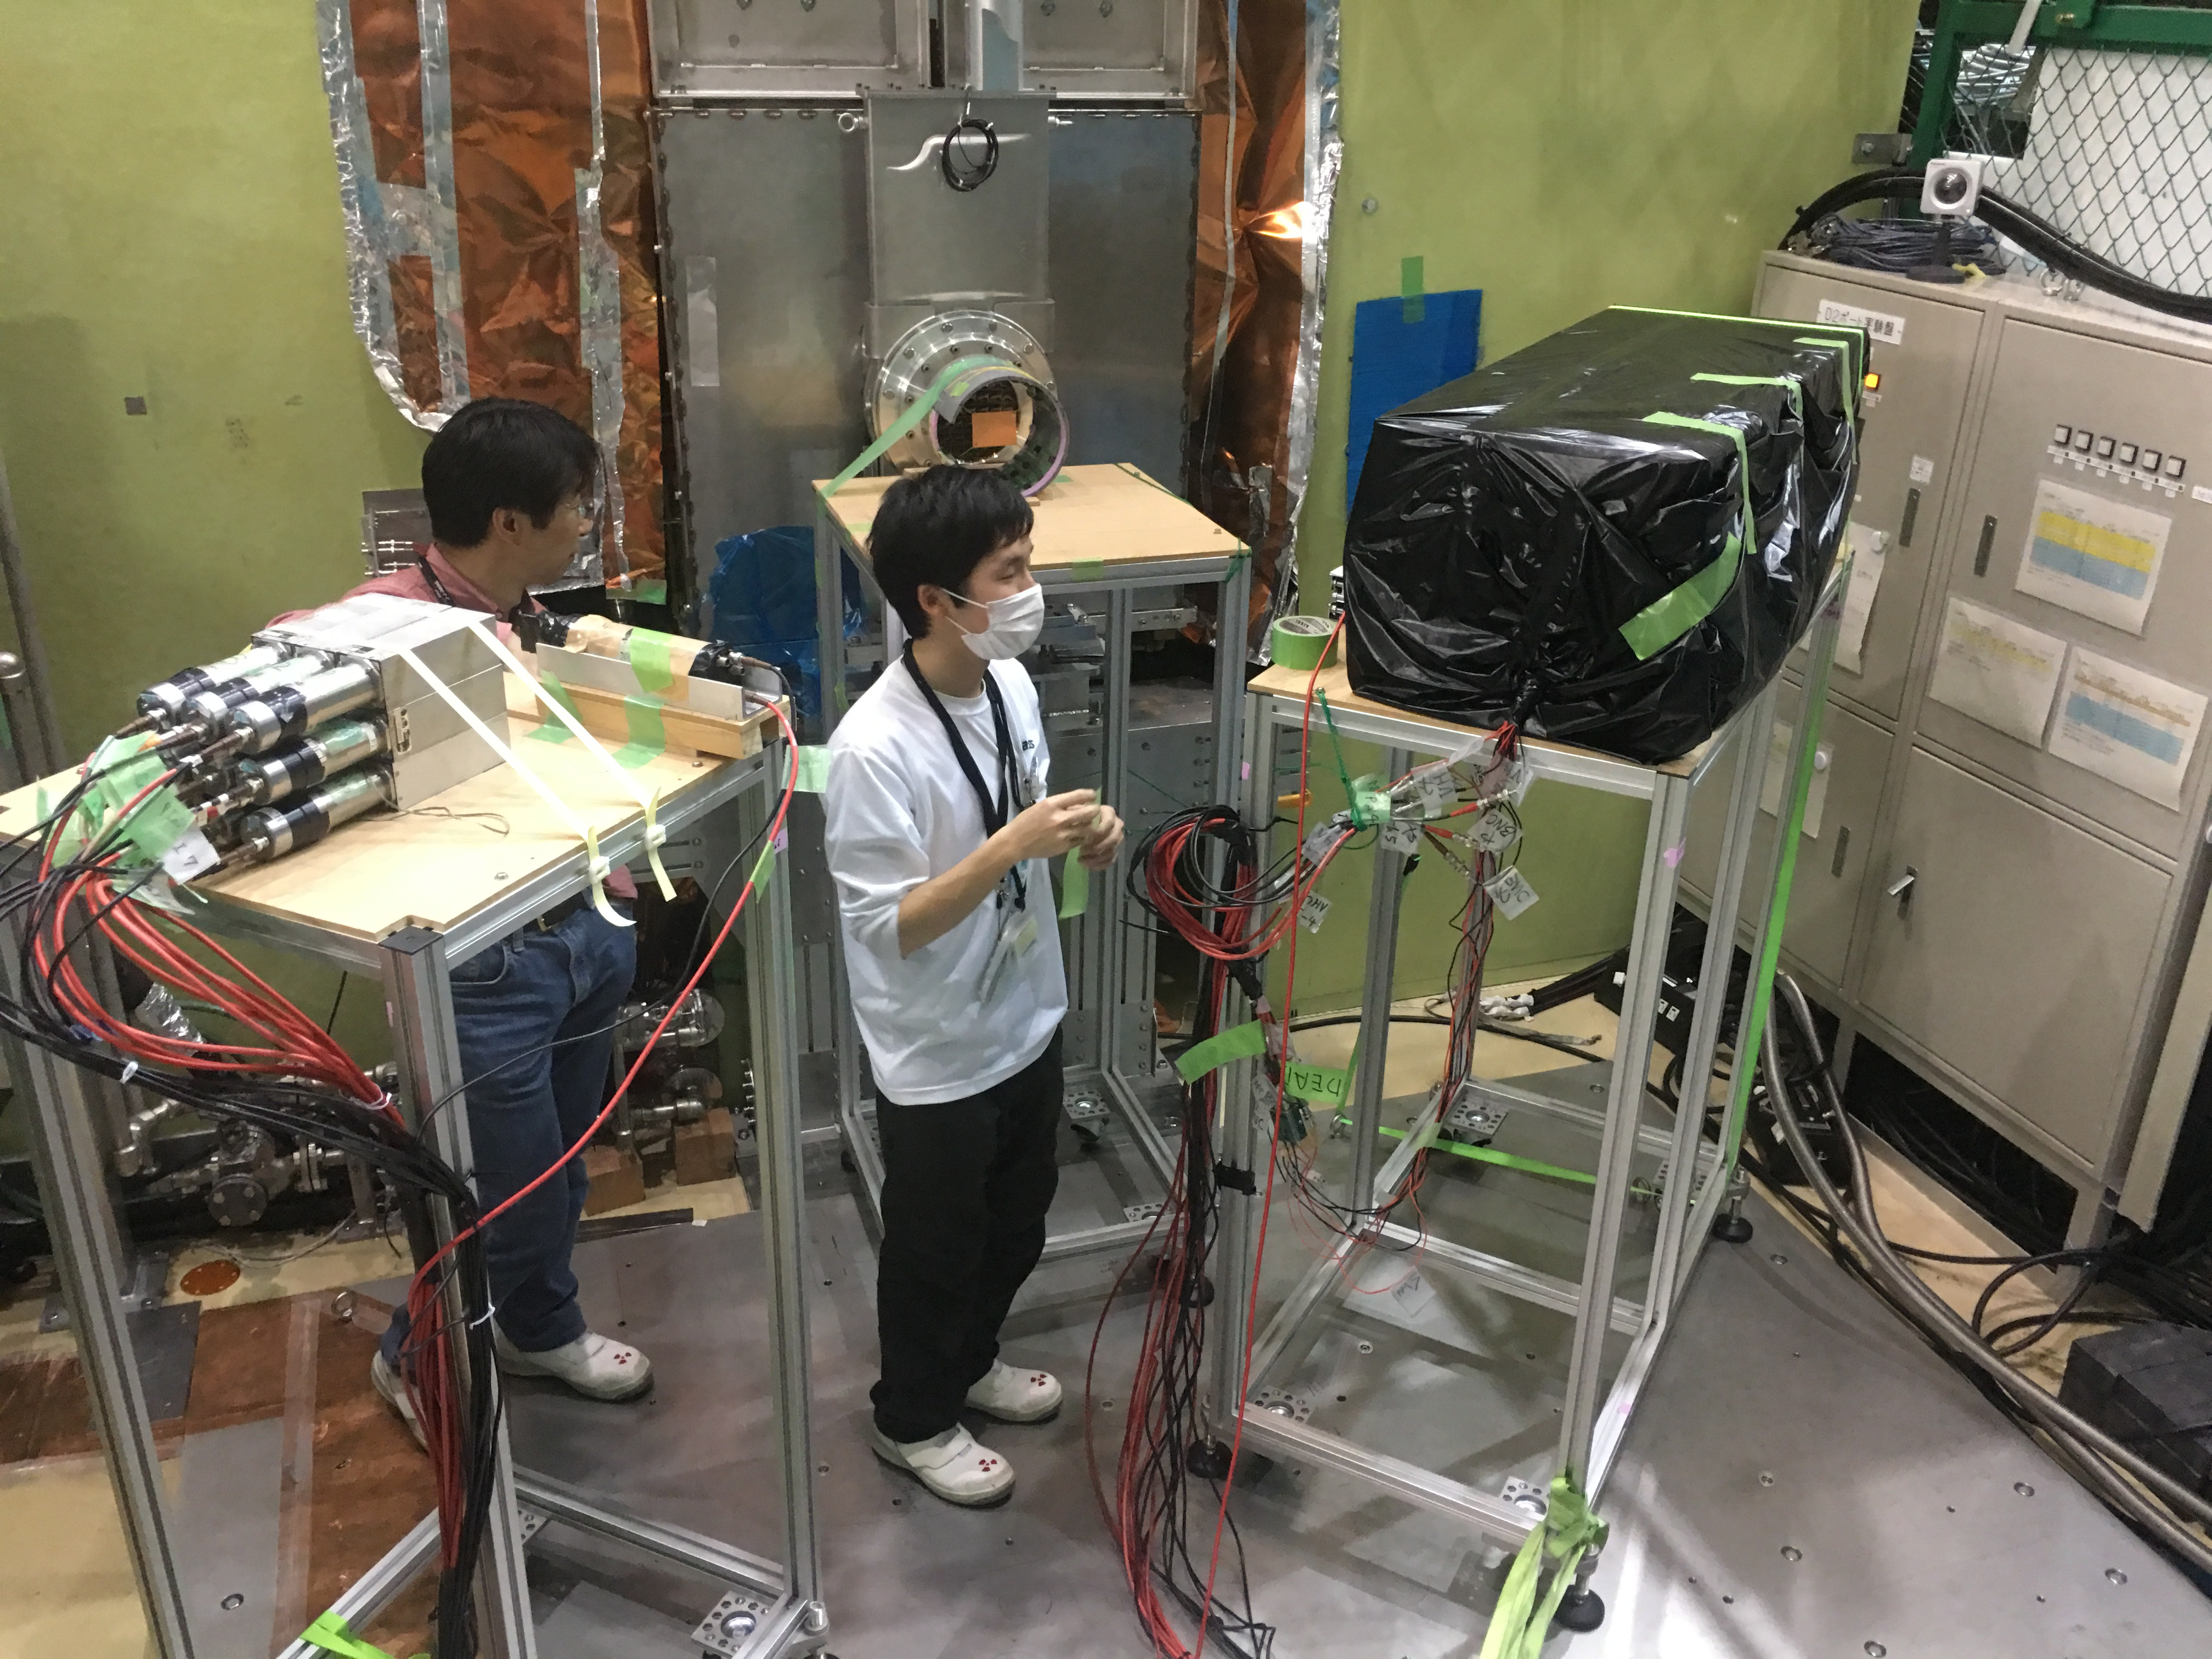
\includegraphics[width=0.5\textwidth]{figure/tajima/g.jpg}
\caption{$g$ 因子測定のセットアップ(写真)}
\label{set_g_2}
\end{figure}

\subsubsection{回路}
この節では本実験の回路について述べる.図~\ref{cir_PS}, \ref{cir_nai}はNaI ,プラスチックシンチレータの回路である.ここでBeam Trigger とは,MLF 施設からの信号のことで,時刻の基準(TO)となっている.これをWFD の外部トリガーとして接続した.また図~\ref{cir_PS}の$n$ - $s \; (n = 1, 2, 3, 4,  s = a, b)$ はプラスチックシンチレータの$n$ 層目のファイバーの片側から読み出される信号を意味する.図中に記載している端子名 (BNC,LEMO,MCX) は接続したケーブルの両端の端子名である.FADC は Waveform Digitizer のことである.
\begin{figure}[H]
\begin{minipage}{0.45\hsize}
\centering
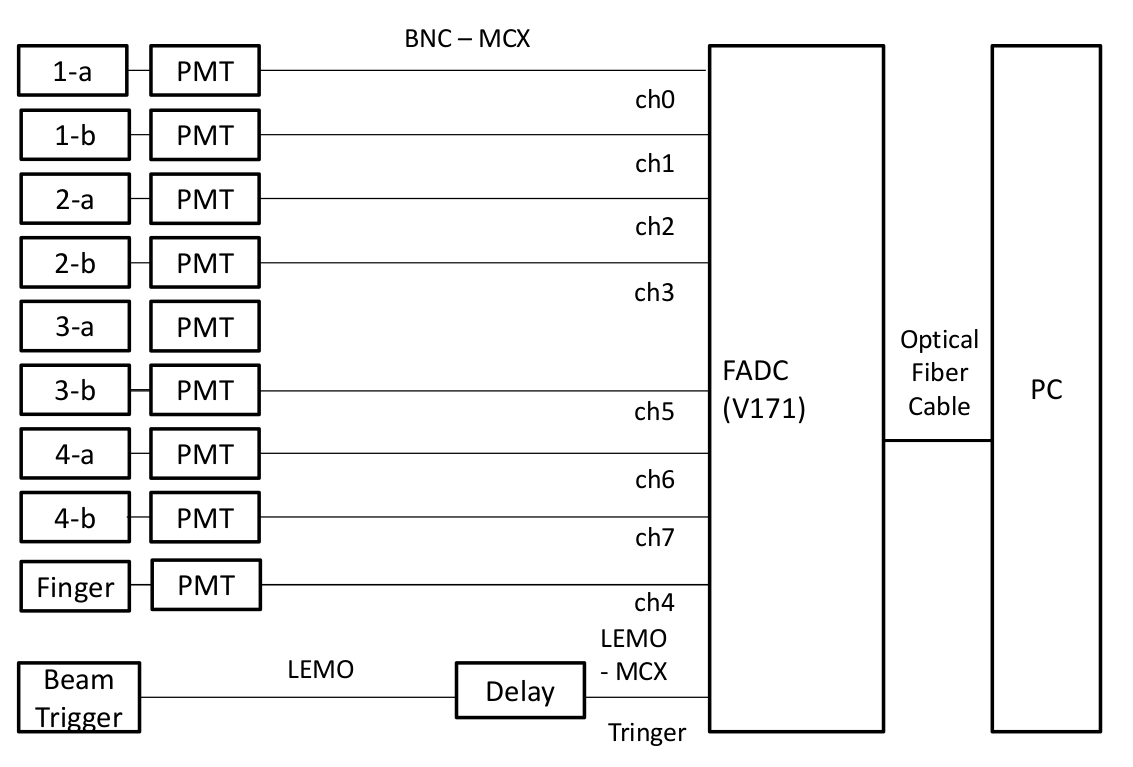
\includegraphics[width=1\textwidth]{figure/tajima/circuit_ps_2.png}
\caption{プラスチックシンチレータ検出器用の回路}
\label{cir_PS}
\end{minipage}
\hfill
\begin{minipage}{0.45\hsize}
\centering
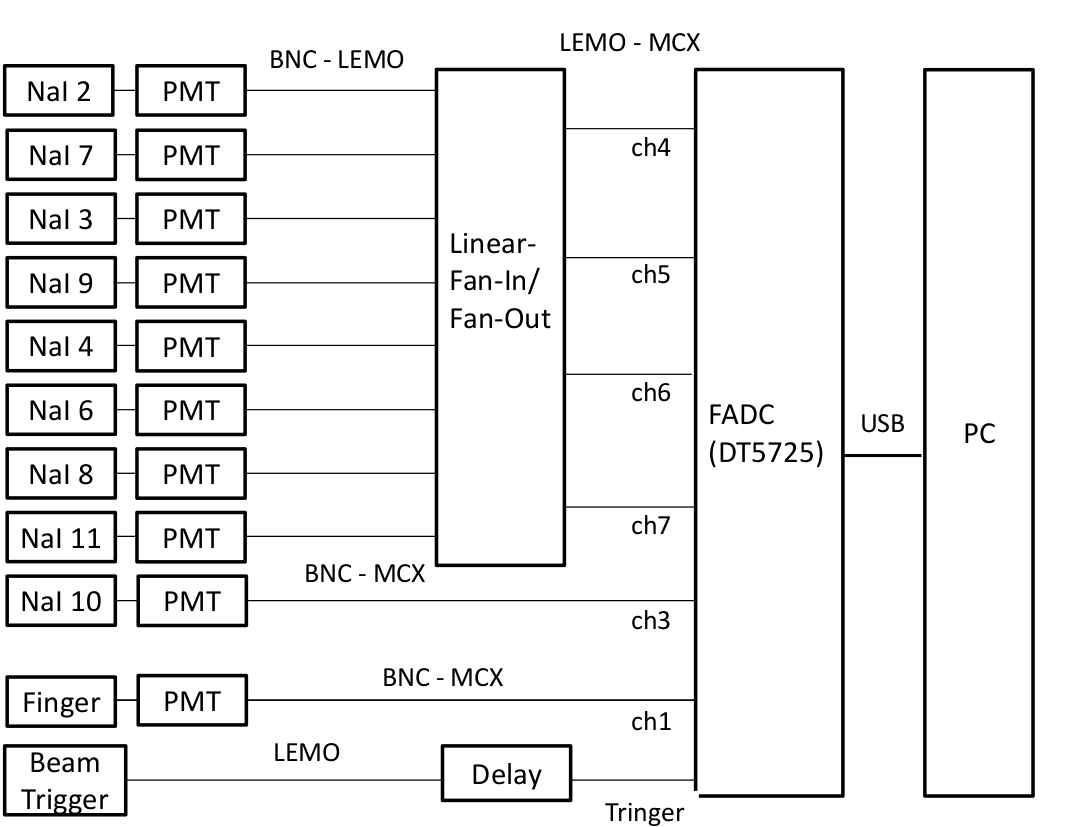
\includegraphics[width=1\textwidth]{figure/tajima/circuit_nai.png}
\caption{NaI 検出器用の回路}
\label{cir_nai}
\end{minipage}
\end{figure}
本実験ではコリメータだけでは不十分で,プラスチックシンチレータにおいても標的から飛んできた陽電子かどうかを判定するためのフィンガーカウンターを設置する必要性が浮上したため,コリメータ前方に設置した.その際にWFD の入力数が不足したため,中間層でありデータとして価値が低いであろうと考えたプラスチックシンチレータの3 層目を片側読み出しにすることにした.

\subsubsection{実験手順}
本実験は以下の手順で行った.
\begin{enumerate}
\item 実験セットアップの調整.
\item ビームが照射される領域に人がいないことを確認し,人が侵入することのないように施錠.
\item ビーム輸送装置上のコリメータを開放し,ビームが標的に照射.
\item コリメーターを制御することで,ビーム1パルス当たりのレートを調整.必要な場合はセットアップを調整.
\item データテイキングを開始.
\end{enumerate}

%\end{document}
